\documentclass[a4paper,UKenglish,cleveref, autoref, thm-restate]{lipicsv2021}
%This is a template for producing LIPIcs articles. 
%See lipics-v2021-authors-guidelines.pdf for further information.
%for A4 paper format use option "a4paper", for US-letter use option "letterpaper"
%for british hyphenation rules use option "UKenglish", for american hyphenation rules use option "USenglish"
%for section-numbered lemmas etc., use "numberwithinsect"
%for enabling cleveref support, use "cleveref"
%for enabling autoref support, use "autoref"
%for anonymousing the authors (e.g. for double-blind review), add "anonymous"
%for enabling thm-restate support, use "thm-restate"
%for enabling a two-column layout for the author/affilation part (only applicable for > 6 authors), use "authorcolumns"
%for producing a PDF according the PDF/A standard, add "pdfa"

%\pdfoutput=1 %uncomment to ensure pdflatex processing (mandatatory e.g. to submit to arXiv)
%\hideLIPIcs  %uncomment to remove references to LIPIcs series (logo, DOI, ...), e.g. when preparing a pre-final version to be uploaded to arXiv or another public repository

%\graphicspath{{./graphics/}}%helpful if your graphic files are in another directory

\bibliographystyle{plainurl}% the mandatory bibstyle

% \title{An Empirical Evaluation of $k$-Means Coresets} %TODO Please add
\title{An Empirical Evaluation of \texorpdfstring{$k$}{k}-Means Coresets} %TODO Please add

%\titlerunning{Dummy short title} %TODO optional, please use if title is longer than one line

\author{Chris Schwiegelshohn}{Department of Computer Science, Aarhus University, Denmark }{schwiegelshohn@cs.au.dk}{[orcid]}{\textcolor{red}{(Optional) author-specific funding acknowledgements}}%TODO mandatory, please use full name; only 1 author per \author macro; first two parameters are mandatory, other parameters can be empty. Please provide at least the name of the affiliation and the country. The full address is optional. Use additional curly braces to indicate the correct name splitting when the last name consists of multiple name parts.

\author{Omar Ali Sheikh-Omar
% \footnote{Optional footnote, e.g. to mark corresponding author}
}{Department of Computer Science, Aarhus University, Denmark}{omar@cs.au.dk}{https://orcid.org/0000-0002-0042-5231}{Innovation Fund Denmark under grant agreement No 0153-00233A.}

\authorrunning{C. Schwiegelshohn and O.A. Sheikh-Omar} %TODO mandatory. First: Use abbreviated first/middle names. Second (only in severe cases): Use first author plus 'et al.'

\Copyright{Chris Schwiegelshohn and Omar Ali Sheikh-Omar} %TODO mandatory, please use full first names. LIPIcs license is "CC-BY";  http://creativecommons.org/licenses/by/3.0/

\ccsdesc[500]{Theory of computation~Data compression}
\ccsdesc[300]{Information systems~Clustering}
%TODO mandatory: Please choose ACM 2012 classifications from https://dl.acm.org/ccs/ccs_flat.cfm 

\keywords{coresets, $k$-means coresets, evaluation, benchmark} %TODO mandatory; please add comma-separated list of keywords

\category{} %optional, e.g. invited paper

\relatedversion{} %optional, e.g. full version hosted on arXiv, HAL, or other respository/website
%\relatedversiondetails[linktext={opt. text shown instead of the URL}, cite=DBLP:books/mk/GrayR93]{Classification (e.g. Full Version, Extended Version, Previous Version}{URL to related version} %linktext and cite are optional

%\supplement{}%optional, e.g. related research data, source code, ... hosted on a repository like zenodo, figshare, GitHub, ...
%\supplementdetails[linktext={opt. text shown instead of the URL}, cite=DBLP:books/mk/GrayR93, subcategory={Description, Subcategory}, swhid={Software Heritage Identifier}]{General Classification (e.g. Software, Dataset, Model, ...)}{URL to related version} %linktext, cite, and subcategory are optional

%\funding{(Optional) general funding statement \dots}%optional, to capture a funding statement, which applies to all authors. Please enter author specific funding statements as fifth argument of the \author macro.

% \acknowledgements{I want to thank \dots}%optional

%\nolinenumbers %uncomment to disable line numbering



%Editor-only macros:: begin (do not touch as author)%%%%%%%%%%%%%%%%%%%%%%%%%%%%%%%%%%
\EventEditors{John Q. Open and Joan R. Access}
\EventNoEds{2}
\EventLongTitle{The European Symposium on Algorithms (ESA)}
\EventShortTitle{ESA 2022}
\EventAcronym{ESA}
\EventYear{2022}
\EventDate{September 2--9, 2022}
\EventLocation{Potsdam, Germany}
\EventLogo{}
\SeriesVolume{42}
\ArticleNo{23}
%%%%%%%%%%%%%%%%%%%%%%%%%%%%%%%%%%%%%%%%%%%%%%%%%%%%%%




% Custom packages

\usepackage{booktabs} % need for table rules
\usepackage{dsfont} % needed for blackboard numbers e.g 11
\usepackage{longtable}
\usepackage{float}


% Custom commands

\newtheorem{fact}[theorem]{Fact}

\newcommand{\R}{\mathbb{R}}
\newcommand{\set}[1]{\{#1\}}
\newcommand{\etal}{et al.\xspace}
\newcommand{\dist}{\text{dist}}
\newcommand{\eps}{\varepsilon}
\newcommand{\opt}{\text{OPT}}
\newcommand{\cost}{\text{cost}}
\newcommand{\calS}{\mathcal{S}}
\newcommand{\calP}{\mathcal{P}}
\newcommand{\calL}{\mathcal{L}}
\newcommand{\calR}{\mathcal{R}}
\newcommand{\calA}{\mathcal{A}}
\newcommand{\calT}{\mathcal{T}}
\newcommand{\ba}{\mathbf{a}}
\newcommand{\bb}{\mathbf{b}}
\newcommand{\bc}{\mathbf{c}}
\newcommand{\bd}{\mathbf{d}}
\newcommand{\bvf}{\mathbf{f}}
\newcommand{\bp}{\mathbf{p}}

\newcommand{\by}{\mathbf{p}}

\newcommand{\E}{\mathbb{E}}
\newcommand{\pr}{\mathbb{P}}
\newcommand{\calE}{\mathcal{E}}
\newcommand{\calI}{\mathcal{I}}
\newcommand{\calF}{\mathcal{F}}
\newcommand{\calX}{\mathcal{X}}
\newcommand{\calB}{\mathcal{B}}
\newcommand{\calC}{\mathcal{C}}
\newcommand{\bI}{\bar{I}_i}
\newcommand{\cand}{\mathbb{C}}
\newcommand{\greedy}{\mathfrak{c}}
\newcommand{\A}{\mathcal{A}}
\newcommand{\poly}{\text{poly}}
\newcommand{\alg}{\greedy}
\newcommand{\centers}{\mathcal{C}}
\newcommand{\coreset}{\Omega}
\newcommand{\offset}{F}
\newcommand{\weight}{f}
\newcommand{\inner}{R_I}
\newcommand{\out}{R_O}
\newcommand{\main}{R_M}
\newcommand{\size}{\Gamma}
\newcommand{\polylog}{\text{polylog}}



\newcommand{\one}{\mathds{1}}

\newcommand{\valuedelta}{\frac{\log^2 1/\eps}{2^{O(z\log z)}\min(\eps^2, \eps^z)}\left(k \log |\cand| + \log \log (1/\eps) + \log(1/\pi)\right)}

\newcommand\chris[1]{\textcolor{blue}{Chris: #1}}
\newcommand\omar[1]{\textcolor{green!60!black}{Omar: #1}}
\newcommand\jesper[1]{\textcolor{yellow!60!black}{Jesper: #1}}



\begin{document}




\maketitle

%TODO mandatory: add short abstract of the document
\begin{abstract}
Coresets are among the most popular paradigms for summarizing data. In particular, there exist many high performance coresets for clustering problems such as $k$-means in both theory and practice. Curiously, there exists no work on comparing the quality of available $k$-means coresets. 

In this paper we perform such an evaluation. There currently is no algorithm known to measure the distortion of a candidate coreset. We provide some evidence as to why this might be computationally difficult.
To complement this, we propose a benchmark for which we argue that computing coresets is challenging and which also allows us an easy (heuristic) evaluation of coresets. Using this benchmark and real-world data sets, we conduct an exhaustive evaluation of the most commonly used coreset algorithms from theory and practice.
\end{abstract}

\newpage

\section{Introduction}

The design and analysis of scalable algorithms has become an important research area over the past two decades. This is particularly important in data analysis, where even polynomial running time might not be enough to handle proverbial \emph{big data} sets.
One of the main approaches to deal with the scalability issue is to compress or sketch large data sets into smaller, more manageable ones. The aim of such compression methods is to preserve the properties of the original data, up to some small error, while significantly reducing the number of data points.

Among the most popular and successful paradigms in this line of research are \emph{coresets}. Informally, given a data set $A$, a coreset $S\subset A$ with respect to a given set of queries $Q$ and query function $f: A\times Q \rightarrow \mathbb{R}_{\geq 0}$ approximates the behaviour of $A$ for all queries up to some multiplicative distortion $D$ via
% $$ \sup_{q\in Q} \max\left( \frac{f(S,q)}{f(A,q)},\frac{f(A,q)}{f(S,q)}\right) \leq D.$$
\begin{equation*}
    \sup_{q\in Q} \max\left( \frac{f(S,q)}{f(A,q)},\frac{f(A,q)}{f(S,q)}\right) \leq D.
\end{equation*}
Coresets have been applied to a number of problems such as computational geometry \cite{AHV05,Chan09}, linear algebra \cite{IndykMGR20,maalouf2019fast}, and machine learning \cite{MRM21,MunteanuSSW18}. But the by far most intensively studied and arguably most successful applications of the coreset framework is the $k$-clustering problem.

Here we are given $n$ points $A$ with (potential unit) weights $w:A\rightarrow \mathbb{R}_{\geq 0}$ in some metric space with distance function $\dist$ and aim to find $k$ centers $C$ such that 
\begin{equation*}
\cost_A(C):= \frac{1}{n} \sum_{p\in A}  \min_{c\in C} w(p)\cdot \dist^z(p,c)
\end{equation*}
is minimized. The most popular variant of this problem is probably the $k$-means problem in $d$-dimensional Euclidean space where $z=2$ and $\dist(x,y) = \sqrt{\sum_{i=1}^d (x_i-y_i)^2}$.

A $(k,\varepsilon)$-coreset is now a subset $\Omega\subset A$ with weights $w:\Omega\rightarrow \mathbb{R}_{\geq 0}$ such that for any set of $k$ centers $C$
\begin{equation}
\label{eq:coreset}
\sup_{C} \max\left( \frac{\cost_A(C)}{\cost_{\Omega}(C)},\frac{\cost_{\Omega}(C)}{\cost_{A}(C)}\right) \leq 1+\varepsilon.
\end{equation}
The coreset definition in \cref{eq:coreset} provides an upper bound for the distortion of all candidate solutions i.e., all possible $k$ clusterings. 
A \emph{weak coreset} is a relaxed guarantee that holds for optimal or nearly optimal clusterings of $A$ instead of all clusterings.

In a long line of work spanning the last 20 years \cite{BecchettiBC0S19,BravermanJKW21,Chen09,FL11,FeldmanSS20,
HaM04,HaK07,huang2020coresets,BravermanJKW21,LS10,SohlerW18}, the size of coresets has been steadily improved with the current state of the art yielding a coreset with $\tilde{O}(k \varepsilon^{-2} \cdot \min(d,\varepsilon^{-2}))$ points for a distortion $D\leq (1+\varepsilon)$ due to Cohen-Addad, Saulpic, and Schwiegelshohn \cite{Cohen-AddadSS21}\footnote{We use $\tilde O(x)$ to hide $\log^c x$ terms for any constant $c$.}.

While we have a good grasp of the theoretical guarantees of these algorithms, our understanding of the empirical performance is somewhat lacking. There exist a number of coreset implementations, but it is usually difficult to assess which implementation summarizes the data best. To accurately evaluate a given coreset, we would need to come up with a $k$ clustering $C$ which results in a maximal distortion. Solving this problem is likely difficult: related questions such as deciding whether a 3-dimensional point set $A$ is an $\varepsilon$-net of a  net of a set $B$ with respect to convex ranges is co-NP hard \cite{GiannopoulosKWW12} and it is similarly co-NP hard to decide whether a point set $A$ is a \emph{weak coreset} of a point set B (see \cref{prop:hardness} in the appendix). 

Due to this difficulty, a common heuristic for evaluating coresets is as follows~\cite{AckermannMRSLS12,FGSSS13}. First, compute a coreset $\Omega$ with the available algorithm(s) using some input data $A$. Then, run an optimization algorithm on $\Omega$ to compute a $k$ clustering $C$. The \emph{best} coreset algorithm is considered to be the one which yields a clustering with the smallest cost.

This practice has substantial drawbacks.
The first is that evaluation method conflates the two separate tasks of coreset construction and optimization.
It is important to note that the first step of virtually all coreset algorithms is a low-cost (bicriteria) constant factor approximation, i.e. a solution with $\beta\cdot k$ clusters that costs at most $\alpha\cdot \opt$, where $\opt$ is the cost of an optimal $k$ clustering.
Given that this initial solution has an $\alpha$ approximation to the cost, a routine calculation shows that the additive error of the coreset, i.e. the maximum difference
$$ \left\vert \cost_A(C) - \cost_B(C) \right\vert $$
over all solutions $C$ is at most $O(\alpha)\cdot \cost_A(C)$. In particular, in the case that the initial bicriteria approximation has $\alpha \ll 2$, which is not too difficult to achieve with more than $k$ centers, all known polynomial time approximation algorithms will find solutions where the additive error $O(\alpha)\cdot \cost_A(C)$ is small compared to error inherent from the approximation algorithm. Thus, it is difficult to measure coreset quality in this way. 

The second drawback is that this practice will typically mainly measure the performance of the optimization algorithm, rather than the performance of the coreset algorithms. If the solution quality of the optimization algorithm is not particularly good, then any coreset algorithm might seem to do well, simply because the optimization algorithm did not encounter any solution with bad guarantees. But even if the solution quality is good, it may not be enough to distinguish solutions that are well approximated from solutions that are not.


The third drawback of this evaluation method is that is does not consider the main use cases of coresets, nor the full power of their guarantee. Indeed, if speeding up the computation of an optimization algorithm, one would hardly need a strong coreset; approximating the cost of every candidate solution, as weaker coreset definitions (or indeed a bicriteria approximation) would be suitable as well. A coresets main and most powerful feature is \emph{composability}, i.e. given two disjoint point sets $X$ and $Y$, the union of a coreset of $X$ and a coreset of $Y$ is a coreset. Composability is what enables coresets to scale to massively parallel computation models and enables simple streaming algorithms via the merge and reduce technique. To which degree a coreset is composable is generally not a property of an optimal clustering of the point set, as optimal solutions $C_X$ of $X$ or $C_Y$ of $Y$ may have little in common with an optimal solution of $X\cup Y$. 


The purpose of this study is to systematically evaluate the quality of various coreset algorithms for $k$-means. As such, we develop a new evaluation procedure which estimates the distortion of coreset algorithms. On real-world data sets, we observe that while the evaluated coreset algorithms are generally able to find solutions with comparable costs, there is a stark difference in their distortions. This shows that differences between optimization and compression are readily observable in practice.

As a complement to our evaluation procedure on real-world data sets, we propose a benchmark framework for generating synthetic data sets. We argue why this benchmark has properties that results in hard instances for all known coreset constructions. We also show how to efficiently estimate the distortion of a candidate coreset on the benchmark.




\section{Coreset Algorithms}
\label{sec:algorithms}

Though the algorithms vary in details, coreset constructions come in one of the following two flavours:
\begin{enumerate}
\item Movement-based constructions: Such algorithms compute a clustering with $T$ points such that $\cost_A(T)\ll \opt$, where $\opt$ is the cost of an optimal $k$-means clustering. The coreset guarantee then follows as a consequence of the triangle inequality. These algorithms all have an exponential dependency on the dimension $d$, and therefore have been overtaken by sampling-based methods. Nevertheless, these constructions are more robust to various constrained clustering formulations~\cite{HuangJV19,SSS19} and continue to be popular. Examples from theory include~\cite{FrahlS2005,HaM04}. 
\item Importance sampling: Points are sampled proportionate to their sensitivity which for a point $p$ is defined as $sens(p):=\sup_{C} \frac{\min_{c\in C} \dist^2(p,c)}{\cost_A(C)}$ and weighted by their inverse sampling probability. In terms of theoretical performance, sensitivity sampling has largely replaced movement based constructions, see for example~\cite{FeldmanL11,LangbergS10}.  
\end{enumerate}

Of course, there exist algorithms that draw on techniques from both, see for example~\cite{Cohen-AddadSS21}. In what follows, we will survey implementations of various coreset constructions that we will evaluate later.


\begin{description}
\item[StreamKM++~\cite{AckermannMRSLS12}] The popular $k$-means++ algorithm~\cite{ArV07} computes a set of centers $K$ by iteratively sampling a point $p$ in $A$ proportionate to $\min_{q\in K} \dist^2(p,q)$ and adding it to $K$. The procedure terminates once the desired number of centers has been reached. The first center is typically picked uniformly at random.
The StreamKM++ paper runs the $k$-means++ algorithms for $T$ iterations, where $T$ is the desired coreset size. At the end, every point $q$ in $K$ is weighted by the number of points in $A$ closest to it. While the construction has elements of important sampling, the analysis is largely movement-based. The provable bound required for the algorithm to compute a coreset is $O\left(\frac{k\log n}{\delta^{d/2}\varepsilon^d}\cdot \log^{d/2} \frac{k\log n}{\delta^{d/2}\varepsilon^d}\right)$.
\item[BICO~\cite{FGSSS13}] Combines the very fast, but poor quality clustering algorithm BIRCH~\cite{ZRL97} with the movement-based analysis from~\cite{FrahlS2005,HaM04}. The clustering is organized by way of a hierarchical decomposition: When adding a point $p$ to one of the coreset points $\Omega$ at level $i$, it first finds the closest point $q$ in $\Omega$. If $p$ is too far away from $q$, a new center is opened at $p$. Otherwise $p$ is either added to $q$, or, if adding $p$ to $q$ increases the clustering cost of $q$ beyond a certain threshold, the algorithm attempts to add $p$ to the child-clusters of $q$. The procedure then continues recursively. The provable bound required for the algorithm to compute a coreset is $O\left(k\varepsilon^{-d-2}\log n\right)$.
\item[Sensitivity Sampling~\cite{FL11}] The simplest implementation of sensitivity sampling first computes an $(O(1),O(1))$ bicriteria $K$ approximation\footnote{An $(\alpha,\beta)$ bicriteria approximation computes an $\alpha$ approximation using $\beta\cdot k$ many centers.}, for example by running $k$-means++ for $2k$ iterations~\cite{Wei16}. Let $K$ be the $2k$ clustering thus computed and let $K_i$ be an arbitrary cluster of $K$ with center $q_i$. Subsequently, the algorithm picks $T-2k$ points proportionate to $\frac{\dist^2(p,q)}{\cost_{K_i}(\{q_i\})} + \frac{1}{|K_i|}$. Let $|\hat{K_i}|$ be the estimated number of points in the sample. Finally, the algorithm weighs each $q_i$ by $(1+\eps)\cdot |K_i| - |\hat{K_i}|$. The provable bound required for the algorithm to compute a coreset is $\tilde O\left(kd\varepsilon^{-4}\right)$ (\cite{FL11}),
$\tilde O\left(k\varepsilon^{-6}\right)$ (\cite{huang2020coresets}), or $\tilde O\left(k^2\varepsilon^{-4}\right)$ (\cite{BravermanJKW21}).
\item[Group Sampling~\cite{Cohen-AddadSS21}] First, the algorithm computes an $O(1)$ approximation (or a bicriteria approximation) $K$. Subsequently, the algorithm preprocesses the input into groups such that (1) for any two points $p,p'\in K_i$, their cost is identical up to constant factors and (2) for any two clusters $K_i,K_j$, their cost is identical up to constant factors. In every group, Group-Sampling now samples points proportionate to their cost. The authors of~\cite{Cohen-AddadSS21} show that there always exist a partitioning into $\log^2 1/\varepsilon$ groups. Points not contained in a group are snapped to their closest center $q$ in $K$. $q$ is weighted by the number of points snapped to it. The provable bound required for the algorithm to compute a coreset is $\tilde O\left(k\varepsilon^{-4}\right)$ (\cite{Cohen-AddadSS21}).
\item[Ray Maker~\cite{harpeled2007raymaker}] The algorithm computes an initial solution with $k$ centers which is a constant factor approximation of the optimal clustering. Around each center, $O(1/\epsilon^{d-1})$ random rays are created which span the hyperplane. Next, each point $p \in A$ is snapped to its closest ray resulting in a set of one-dimensional points associated with each ray. Afterwards, a coreset is created for each ray by computing an optimal 1D clustering with $k^2/\epsilon^2$ centers and weighing each center by the number of points in each cluster. The final coreset is composed of the coresets computed for all the rays.
The provable bound required for the algorithm to compute a coreset is $O(n + \text{poly}(k,\log n, 1/\epsilon) + \text{func}(k, \epsilon))$ where $\text{poly}$ is a polynomial and $\text{func}(k,\epsilon)$ is a function which depends on $k$ and $\epsilon$. The algorithm has recently received some attention due to its applicability to the fair clustering problem~\cite{HuangJV19}.
\end{description}

\subsection{Dimension Reduction}
\label{sec:dim_reduction}

Finally, we also combine coreset constructions with a variety of dimension reduction techniques. Since the seminal paper by Feldman, Schmidt, and Sohler~\cite{FSS13}, most coreset algorithms have used some form of dimension reduction to eliminate the dependency on $d$, either by explicitly computing a low-dimensional embedding, see for example~\cite{FSS13,SoW18}, or by using the existence of a suitable embedding in the analysis~\cite{Cohen-AddadSS21,huang2020coresets}.

In particular, movement-based coresets often have an exponential dependency on the dimension, which can be alleviated with some form of dimension reduction, both in theory~\cite{SSS19} and in practice~\cite{KappmeierS015}.
Here the are two main techniques.

\begin{description}
\item[Principal Component Analysis:] Feldman, Schmidt, and Sohler~\cite{FSS13} showed that projecting an input $A$ onto the first $O(k/\varepsilon^2)$ principal components is a coreset, albeit in low dimension. The analysis was subsequently tightened by~\cite{CEMMP15} and extended to other center based cost functions by~\cite{SohlerW18}. Although its target dimension is generally worse than those based on random projections and terminal embeddings, there is nevertheless reasons for using PCA regardless: It removes noise and thus may make it easier to compute a high quality coreset.
\item[Terminal Embeddings:] Given a set of points $A$ in $\mathbb{R}^d$, a terminal embedding $f:\mathbb{R}^d\rightarrow \mathbb{R}^m$ preserves the pairwise distance between any point $p\in A$ and any point $q\in \mathbb{R}^d$ up to a $(1\pm \varepsilon)$ factor. The statement is related to the famous Johnson-Lindenstrauss lemma but it is stronger as it does not apply to only the pairwise distances of $A$. Nevertheless, the same target dimension is sufficient. Terminal embeddings were studied by~\cite{ElkinFN17,MahabadiMMR18,NaN18}, with Narayanan and Nelson \cite{NaN18} achieving an optimal target dimension of $O(\varepsilon^{-2}\log n)$, where $n$ is the number of points. For applications to coresets, we refer to \cite{BecchettiBC0S19,Cohen-AddadSS21,huang2020coresets}.
\end{description}

For an overview on practical aspects of dimension reduction, we refer to Venkatsubramanian and Wang~\cite{VenkatasubramanianW11}. In our evaluation, we  focus on using PCA. The performance of the algorithms when applying a Johnson-Lindenstrauss transformation does not affect the behaviour of an algorithm that only depends on pairwise distances. We note that terminal embeddings, combined with an iterative application of the coreset construction from \cite{BravermanJKW21}, can reduce the target dimension to a factor $\tilde{O}(\varepsilon^{-2} \log k)$. This is mainly of theoretical interest, as in practice the deciding factor wrt the target dimension is the precision, rather than dependencies on $\log n$ and $\log k$.

\section{Benchmark Construction}
\label{sec:benchmark}

In this section, we describe our benchmark. The benchmark has a parameter $\alpha$ which controls the number of points and dimensions of the generated data instance.
For a given value of $k$, the benchmark instance consists of $n=k^\alpha$ points and $d=\alpha \cdot k$ dimensions. A benchmark instance is a $n\times d$ matrix $A$ which is recursively constructed as follows.

Let $\one_k$ be the $k$-dimensional all-one vector and $v_i^1$ be the $k$-dimensional vector with entries $(v_i^1)_j = \begin{cases}-\frac{1}{k} & \text{if } i\neq j\\
\frac{k-1}{k} & \text{if } i= j\end{cases}$.
For $\ell\leq \alpha$, recursively define the $k^{\ell}$ dimensional vector $v_i^{\ell} = \begin{bmatrix}
(v_i^{\ell-1})_1 \cdot \one_k \\
(v_i^{\ell-1})_2 \cdot \one_k \\
\vdots \\
(v_i^{\ell-1})_1 \cdot \one_k
\end{bmatrix}$. 
Finally, set the $t$-th column of $A$, for $t = a\cdot k + b$, $a\in \{0,\ldots \alpha-1\}$ and $b \in \{1,\ldots k\}$, to be $k^{\alpha-a+1}$  stacks of $v_b^{a+1}$.


To get a better feel for the construction, we have given two small example instances for $k=2$ and $k=3$ in the appendix (see \cref{fig:benchmark-small-instances}).


\subsection{Properties of the Benchmark}

We now summarize the key properties of the benchmark.
To this end, we require a few notions.
Let $A$ be the input matrix. We slightly abuse notation and refer to $A_i$ as both the $i$th point as well as the $i$th row of the matrix $A$.
For a clustering $\mathcal{C}=\{C_1,\ldots ,C_k\}$, we define that the $n\times k$ indicator matrix $\tilde X$ induced by $\mathcal{C}$ via
\begin{align*}
\tilde X_{i,j} = \begin{cases}1 & \text{if } A_i\in C_j \\
0 & \text{else.} \end{cases} 
\end{align*}
Furthermore, we will also use the $n\times k$ normalized clustering matrix $ X$ defined as
\begin{align*}
X_{i,j} = \begin{cases}\frac{1}{\sqrt{|C_i|}} & \text{if } A_i\in C_j \\
0 & \text{else.} \end{cases}    
\end{align*}
We also recall the following lemma which will allow us to express the $k$-means cost of a clustering $\mathcal{C}$ with optimally chosen centers in terms of the cost of $X$ and $A$.
\begin{lemma}[Folklore]
\label{lem:magic}
Let $A$ be an arbitrary set of points and let $\mu(A) = \frac{1}{|A|}\sum_{p\in A} p$ be the mean. Then for any point $c$
\begin{align*}
 \sum_{p\in A} \|p-c\|^2 = \sum_{p\in A} \|p-\mu(A)\|^2 + |A|\cdot \|\mu(A)-c\|^2.
\end{align*}
\end{lemma}
This lemma proves that for any given cluster $C_j$, the mean is the optimal choice of center. 
We also note that any two distinct columns of $X$ are orthogonal. Furthermore $\frac{1}{n}\mathbf{1}\mathbf{1}^TA$ copies the mean into every entry of $A$. Combining these two observations, we see that the matrix $XX^TA$ maps the $i$th row of $A$ onto the mean of the cluster it is assigned to. Finally, define the Frobenius norm of an $n\times d$ $A$ by $\|A\|_F = \sqrt{\sum_{i=1}^n\sum_{j=1}^d A_{i,j}^2}$. Then the $k$-means cost of the clustering $\mathcal{C}$ is precisely
$\|A-XX^TA\|_F^2.$

We also require the following distance measure on clusterings as proposed by Meila~\cite{Meila05,Meila06}. Given two clusterings $\mathcal{C}$ and $\mathcal{C'}$, the $k\times k$ confusion matrix $M$ is defined as
$ M_{i,j} = |C_i\cap C'_j|.$
Furthermore for the indicator matrices $\tilde X$ and $\tilde X'$ induced by $\mathcal{C}$ and $\mathcal{C'}$ we have the identity $M=\tilde X^T {\tilde X'}$.
Denote by $\Pi_k$ the set of all permutations over $k$ elements. Then the distance between  $\mathcal{C}$ and $\mathcal{C'}$ is defined as
\begin{align*}
d(\mathcal{C},\mathcal{C'}) = 1-\frac{1}{n}\underset{\pi\in \Pi_k}{\max} \sum_{i=1}^k M_{i,\pi(i)}.
\end{align*}
Observe that for clusters that are identical, their distance is $0$. The maximum distance between any two $k$ clusterings is always $\frac{k-1}{k}$.


We are now ready to state the desired properties of our benchmark. The benchmark was designed to generate many clusterings such that
\begin{enumerate}
\item The distance between these clustering is $1-\frac{1}{k}$, i.e. it is maximized.
\item The clusterings have equal cost and the centers in each clustering have equal cost.
\item The clusterings are induced by a set of centers in $\mathbb{R}^d$.
\end{enumerate}

A formal verification of these properties can be found in the appendix.
The first and second property ensure that (equally good) solutions we use for evaluation are spread out through the solution space. In other words, we are less likely to only focus on a set of solutions $\mathcal{S}$ for which a low distortion on one $S\in\mathcal{S}$ implies a low distortion for all elements of $\mathcal{S}$.
The third property is important as these are the only clusterings the (standard) coreset guarantee has to apply to. 

The solutions we consider are given as follows. For the columns $a\cdot k+1,\ldots (a+1)\cdot k$, we define the clustering $\mathcal{C}^{a} = \{C_1^a,\ldots C_k^a\}$ with 
$A_i\in C_j^a$ if and only if $A_{i,j} > 0$. Let $\tilde X^a$ and $X^{a}$ denote the indicator matrix and clustering matrix, respectively, as induced by $\mathcal{C}^{a}$.



\subsection{Benchmark Evaluation}

We now describe how we use the benchmark to measure the distortion of a coreset. Assume that the coresets only consists of input points\footnote{It is not necessary for coreset constructions in general to consists of input points. One can adjust the evaluation in to account for this. But since all algorithms considered in this paper have the property and it makes the evaluation simpler, we will only consider coresets that are subsets of the original point set.}.

Consider the clustering $\mathcal{C}^{a} = \{C_1^a,\ldots C_k^a\}$ for some $a$ and let $\Omega$ with weights $w:\Omega\rightarrow \mathbb{R}_{\geq 0}$ be the coreset. 
Note that there are $\alpha$ many such clusterings, for each value of $a$.
We use $w(C_i^a \cap \Omega):=\sum_{p\in C_i^a \cap \Omega} w(p)$ to denote the mass of points of $C_i^a$ in $\Omega$.
For every cluster $C_i^a$ with $w(C_i^a \cap \Omega)\geq |C_i| (1-\varepsilon)$, we place a center at $\mu(C_i^a)$. Conversely, if $w(C_i^a \cap \Omega)< |C_i^a| (1-\varepsilon)$, we do not place a center at $\mu(C_i^a)$. We call such clusters \emph{deficient}. Let $\calS$ be the total number of thus placed centers.

We now compare the cost as computed on the coreset and the true cost of $\calS$. Due to \cref{lem:magic} and the fact that all clusters have equal cost, we may write for any deficient cluster $C_i^a$
$\cost_{C_i^a}(\calS) = \cost_{C_j^a}(\{\mu(C_j^a)\}) + k^{\alpha-1}\|\mu(C_j^a)-\mu(C_h^a)\|_2^2$, where $C_h^a$ is a non-deficient cluster.
Thus, the cost is 
\begin{eqnarray*}
\cost_{C_i^a}(\calS) &\approx & (1+\frac{2}{\alpha})\cdot \cost_{C_j^a}(\{\mu(C_j^a)\}).
\end{eqnarray*}

Conversely, the cost on the coreset is
\begin{eqnarray*}
\cost_{\Omega\cap C_i^a}(\calS)  
%&= &w(C_i^a \cap \Omega)\left((\alpha-1)\cdot \left(\left(\frac{k-1}{k}\right)^2 + (k-1)\left(\frac{1}{k}\right)^2\right) + 2\right) \\
& \approx & \frac{w(C_i^a \cap \Omega)}{ \cost_{C_j^a}(\{\mu(C_j^a)\})}(1+\frac{2}{\alpha})\cdot \cost_{C_j^a}(\{\mu(C_j^a)\}).
\end{eqnarray*}
Thus for each deficient clustering individually, the distortion will be close to $\frac{k^{\alpha-1}}{w(C_i^a \cap \Omega)} \geq \frac{1}{1-\varepsilon}$.
If there are many deficient clusters, then this will also be the overall distortion.
For all possible (suitably discritized) thresholds for deficiency, we can now identify the clustering $\mathcal{C}^a$ with a maximum number of deficient clusters and use the aforementioned construction to get a lower bound on the distortion.


\subsection{Further Extensions}

On the benchmark we considered here, both Sensitivity Sampling, as well as Group Sampling are similar to uniform sampling and, indeed, uniform sampling could be used to construct a good coreset. We can eliminate uniform sampling as a viable algorithm for this instance by combining multiple benchmarks $B_1,\ldots B_t$ with $\sum_{i=1}^t  k_i =k$. Each benchmark then has size $\sum_{i=1}^t  k_i^{\alpha}$. We then add an additive offset to the coordinates of each benchmark such that they do not interfere. In this case, uniform sampling does not work if the values of the $k_i$ are different enough. Since it is well known that uniform sampling is not a viable coreset algorithm in both theory and practice, we only used the basic benchmark for our evaluations.




\section{Experiments} \label{sec:experiments}
In this section, we describe our experimental evaluation of four widely used algorithms on real-world datasets and our benchmark. The goal is to assess the quality of the generated $k$-means coresets. On that account, we measure the distortion. In addition, we want to measure how noise reduction affects the coreset quality. For that, we create PCA transformed version for each of the real-world datasets. As the evaluated algorithms are randomized, we repeat each experiment ten times, reporting the mean distortion and cost.


\subsection{Datasets}
We use three common real-world datasets for evaluating $k$-means coresets 
---
\textit{Census}\footnote{\url{https://archive.ics.uci.edu/ml/datasets/US+Census+Data+(1990)}},
\textit{Covertype}\footnote{https://archive.ics.uci.edu/ml/datasets/covertype}, and 
\textit{Tower}\footnote{\url{http://homepages.uni-paderborn.de/frahling/coremeans.html}}
---
and several instances of the proposed benchmark. 
The \textit{Census} dataset is a small subset of the Public Use Microdata Samples from 1990 US census. It consists of demographic information encoded as 68 categorical attributes of 2,458,285 individuals. \textit{Covertype} is comprised of cartographic descriptions and forest cover type of four wilderness areas in the Roosevelt National Forest of Northern Colorado in the US. It consists of 581,012 records, 54 cartographic variables and one class variable. Although \textit{Covertype} was originally made for classification tasks, it is often used for clustering tasks by removing the class variable~\cite{AckermannMRSLS12}. \textit{Tower} is a 2,560 by 1,920 picture of a tower on a hill where each pixel is represented by a RGB color value. This dataset consists of 4,915,200 rows and 3 columns. To evaluate how denoising effects the quality of the output, we apply SVD on \textit{Census} and \textit{Covertype} using the $k$ largest singular values. Note that we do not reduce the number of dimensions of the original datasets. As for the benchmark dataset, instances are generated to match roughly the sizes of the real-world datasets. The chosen parameters values and the corresponding dataset sizes are shown in ~\cref{tab:benchmark-instances-overview}. 
% We generated a set of instances with no scaling i.e., $\beta=1.0$ (referred to as \textit{Benchmark-1.0}) and with maximum scaling; $\beta = 2.0$ (\textit{Benchmark-2.0}).




%
\begin{table}
	\begin{center}%\centering
	\caption{The sizes of the real-world datasets used for the experimental evaluation}
	\label{tab:real-world-datasets-overview}
% 	\resizebox{\textwidth}{!}{
	\begin{tabular}{lrr}
		\toprule
        
		    & Data points
		    & Dimensions
            \\
		\midrule
		\textit{Census}
    		& 2,458,285
    		& 68
    		\\
	    \textit{Covertype}
    	    & 581,012
    		& 54
    		\\
        \textit{Tover}
            & 4,915,200
    		& 3
    		\\
		\bottomrule
	\end{tabular}\\
	\end{center}
% 	}
\end{table}



%
\begin{table}
	\begin{center}%\centering
	\caption{The parameter values and the sizes of the benchmark instances used for the experimental evaluation.}
	\label{tab:benchmark-instances-overview}
% 	\resizebox{\textwidth}{!}{
	\begin{tabular}{rrrr}
		\toprule
        $k$
		    & $\alpha$
		    & Data points
		    & Dimensions
            \\
		\midrule
        10
    		& 6
    		& 1,000,000
    		& 60
    		\\
        20
    		& 5
    		& 3,200,000
    		& 100
    		\\
        30
    		& 4
    		& 810,000
    		& 120
    		\\
        40
    		& 4
    		& 2,560,000
    		& 160
    		\\
    %     50
    % 		& 4
    % 		& 6,250,000
    % 		& 200
    % 		\\
		\bottomrule
	\end{tabular}\\
	\end{center}
% 	}
\end{table}

\subsection{Algorithm Parameters}
We followed the same experimental procedure with respect to the choice of parameter values for the algorithms as prior works~\cite{FGSSS13, AckermannMRSLS12}. For the target coreset size, we used $200k$ for all our experiments. On \textit{Census} and \textit{Covertype}, we used $k$ values $\{10, 20, 30, 40, 50\}$, while for \textit{Tower} we used larger cluster sizes $k \in \{20, 40, 60, 80, 100\}$ as in. On the benchmark instances, we settled on $k \in \{10, 20, 30, 40\}$ as a reasonable trade-off between running time and dataset size.



\subsection{Results}

\begin{figure*}
  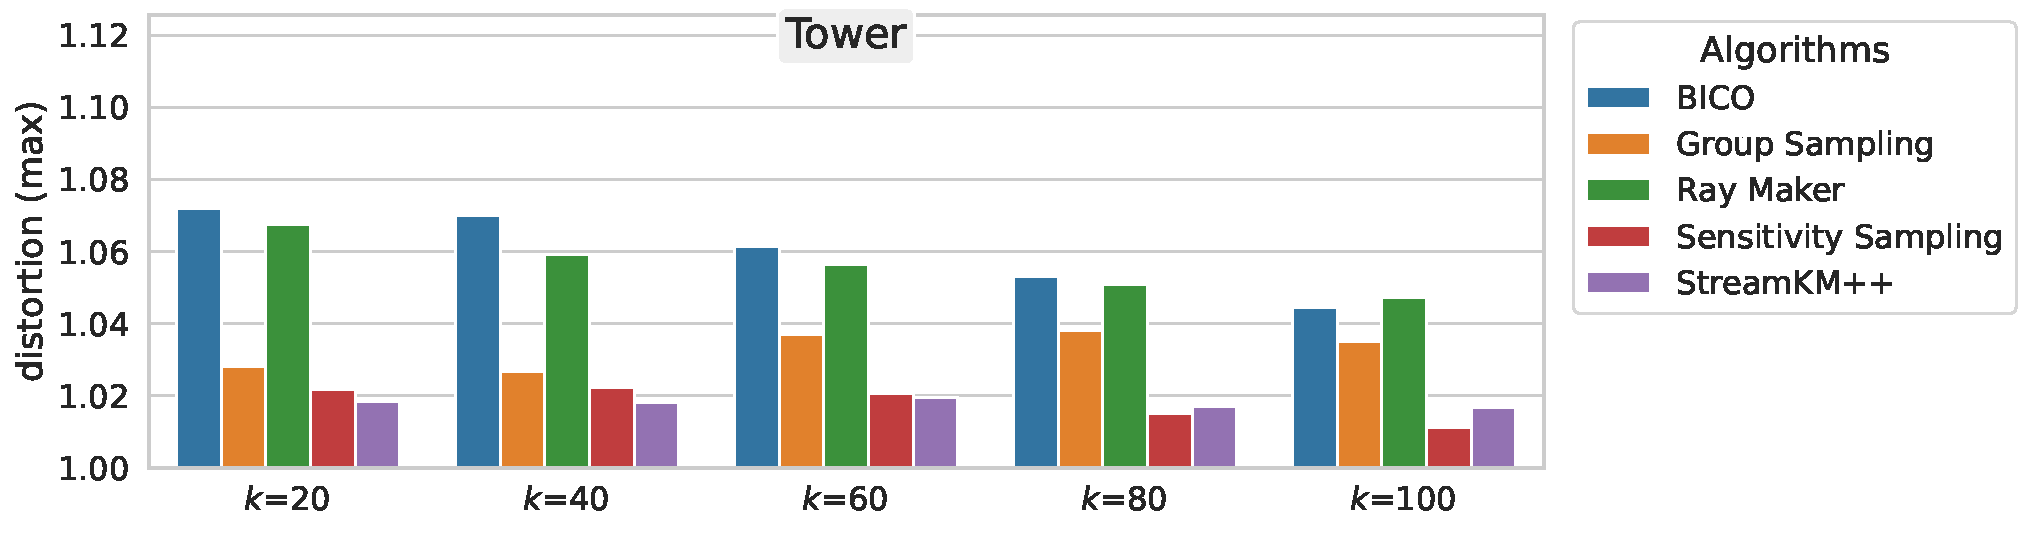
\includegraphics[width=.65\linewidth]{figures/distortions-Tower.pdf}
  \newline \newline
  \subfloat{
    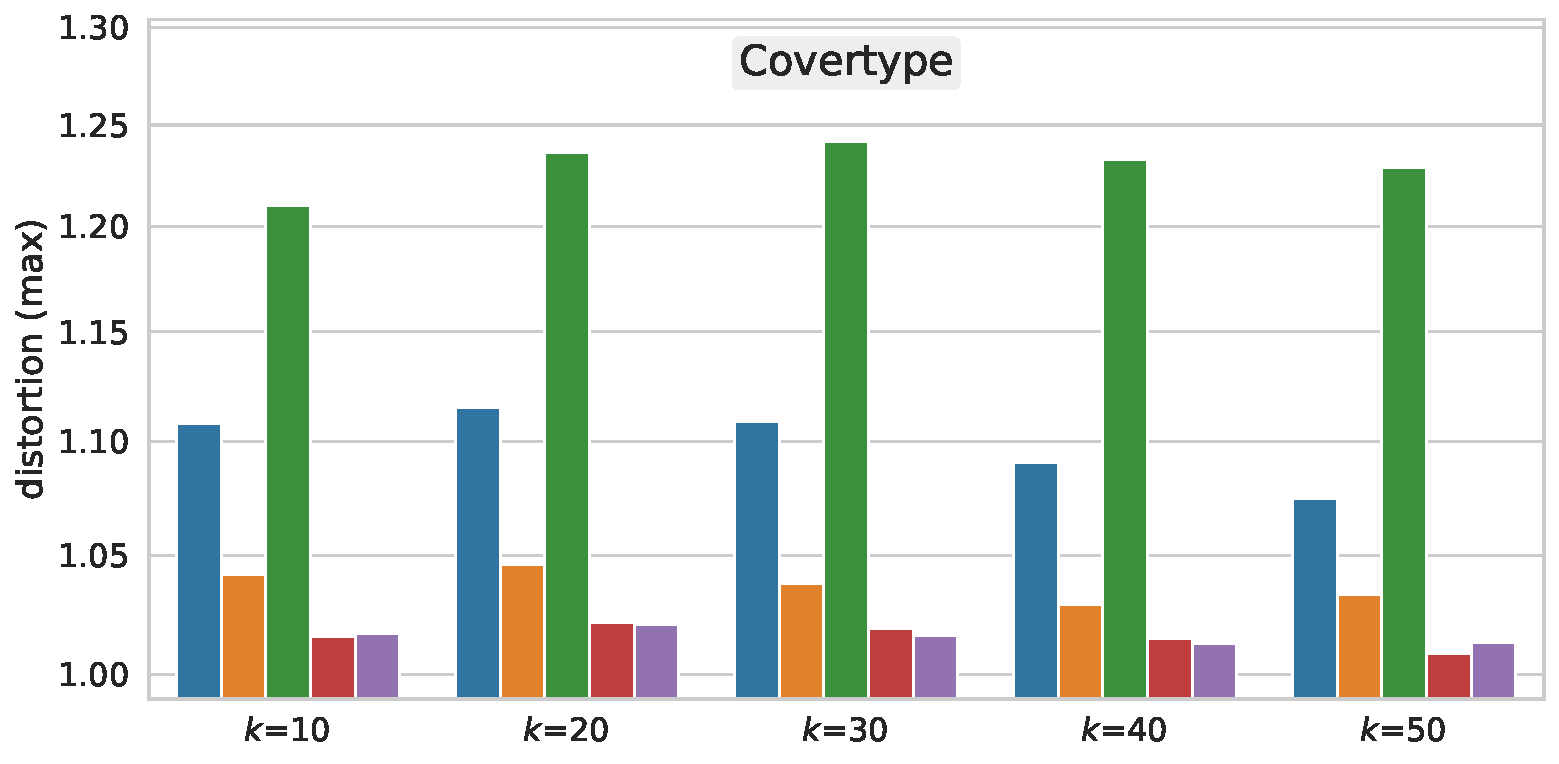
\includegraphics[width=0.5\textwidth]{figures/distortions-Covertype.pdf}
  }
  \subfloat{
    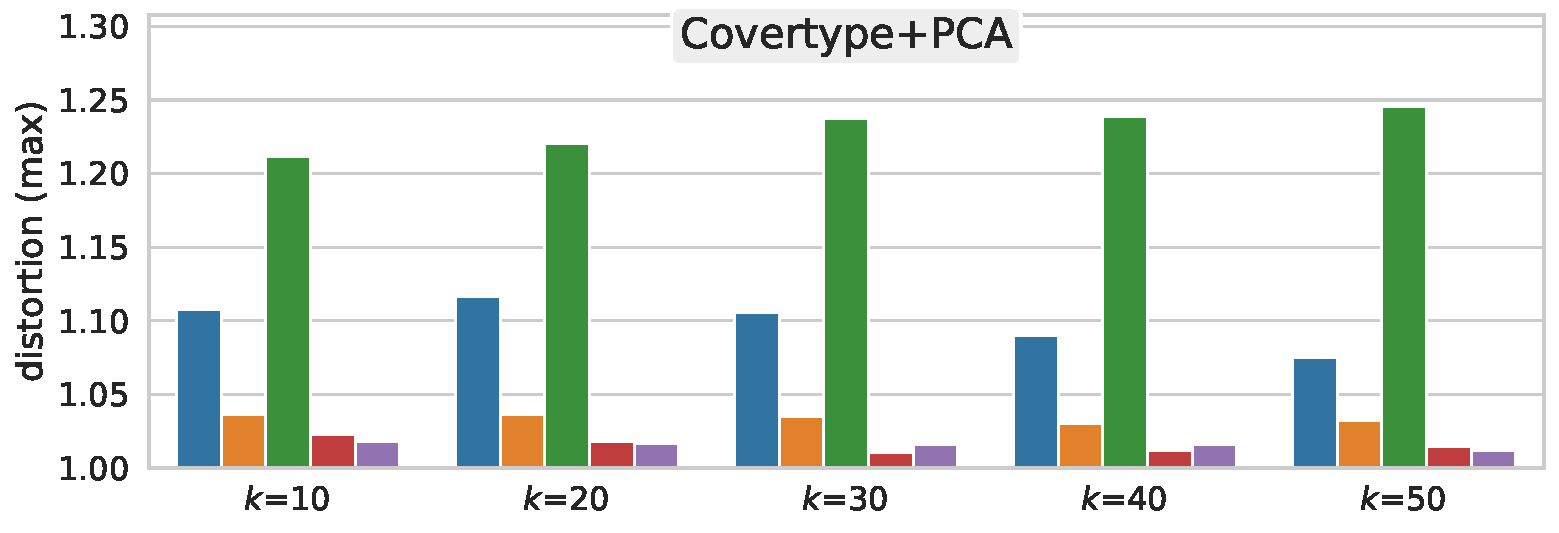
\includegraphics[width=.5\linewidth]{figures/distortions-Covertype+PCA.pdf}
  }
  \newline \newline
  \subfloat{
    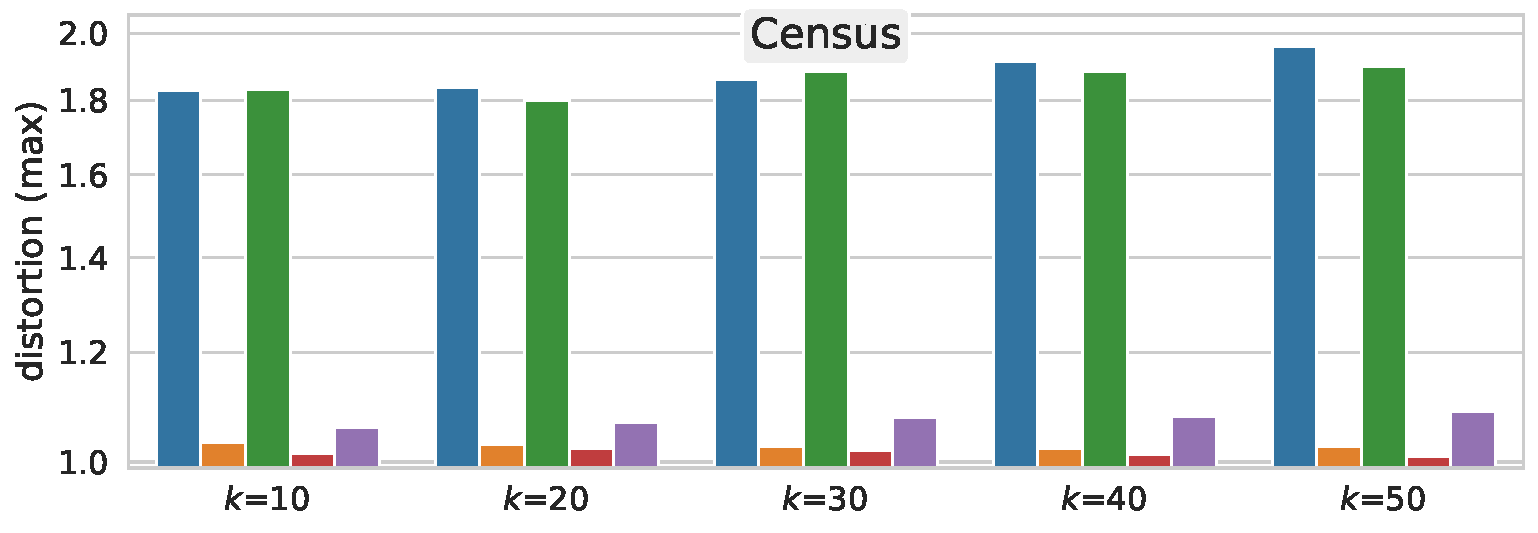
\includegraphics[width=0.5\textwidth]{figures/distortions-Census.pdf}
  }
  \subfloat{
    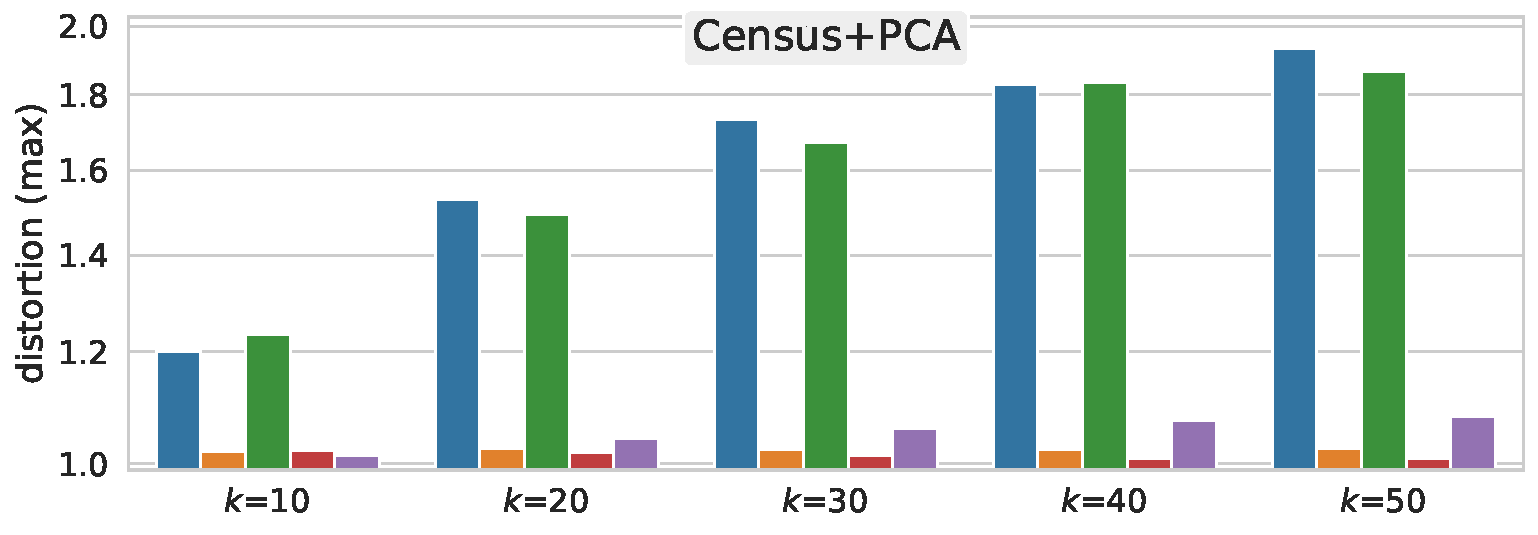
\includegraphics[width=.5\linewidth]{figures/distortions-Census+PCA.pdf}
  }
  \newline \newline
  \subfloat{
    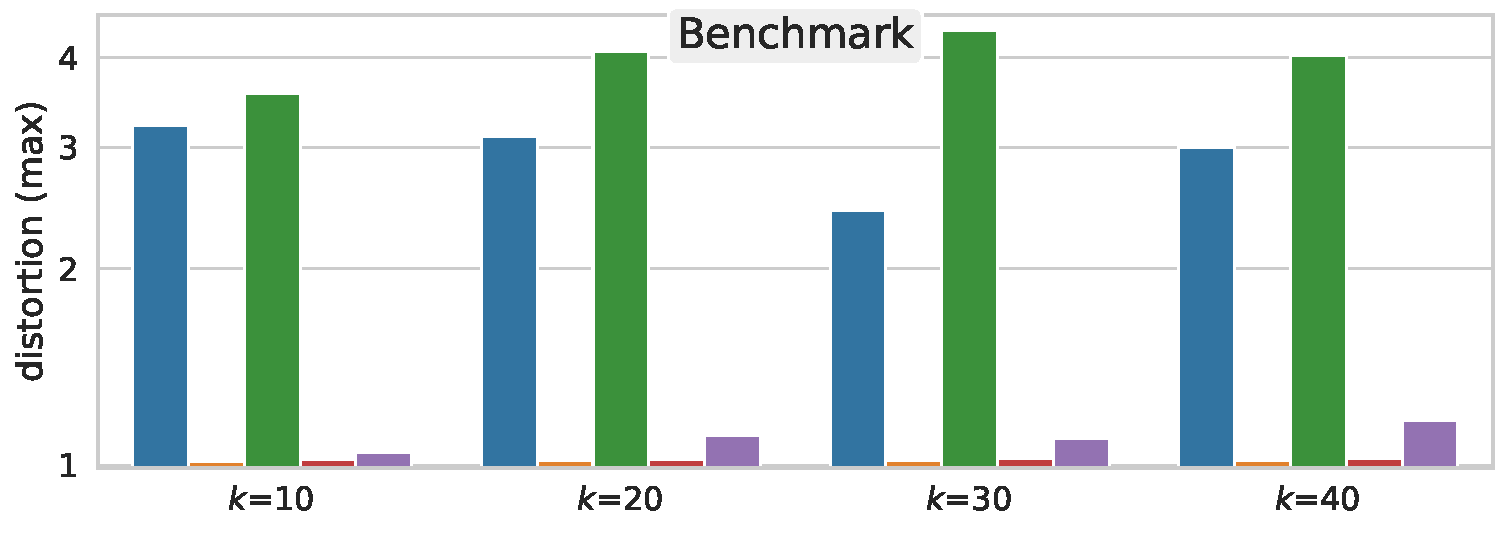
\includegraphics[width=0.5\textwidth]{figures/distortions-Benchmark.pdf}
  }
%   \subfloat{
%     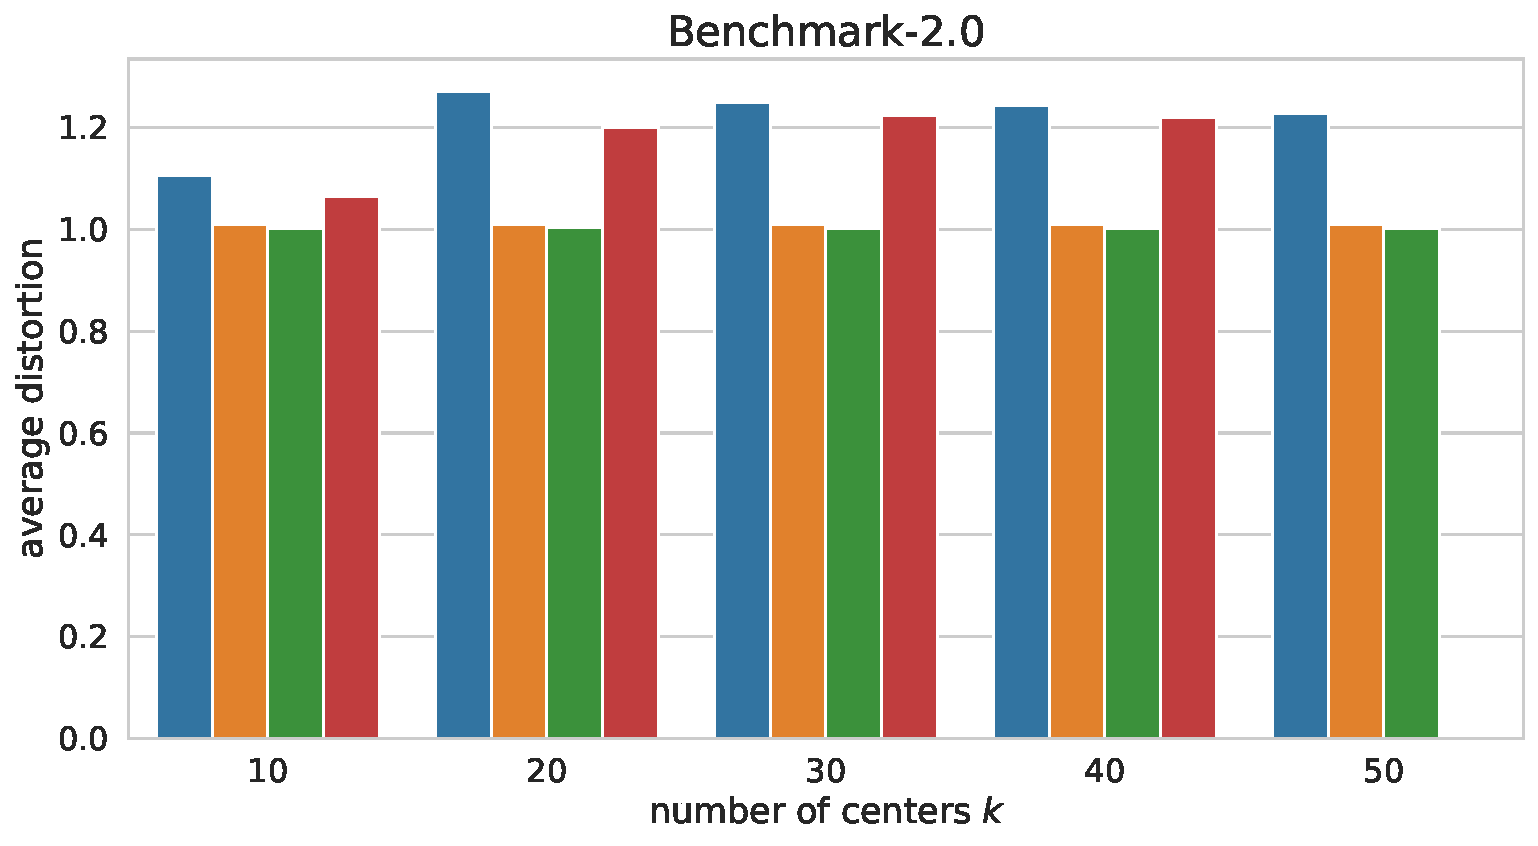
\includegraphics[width=.5\linewidth]{figures/results-Benchmark-2.0.pdf}
%   }
  \label{fig:results}
  \caption{The average distortion of the evaluated algorithms on different datasets.}
\end{figure*}




\begin{figure*}
  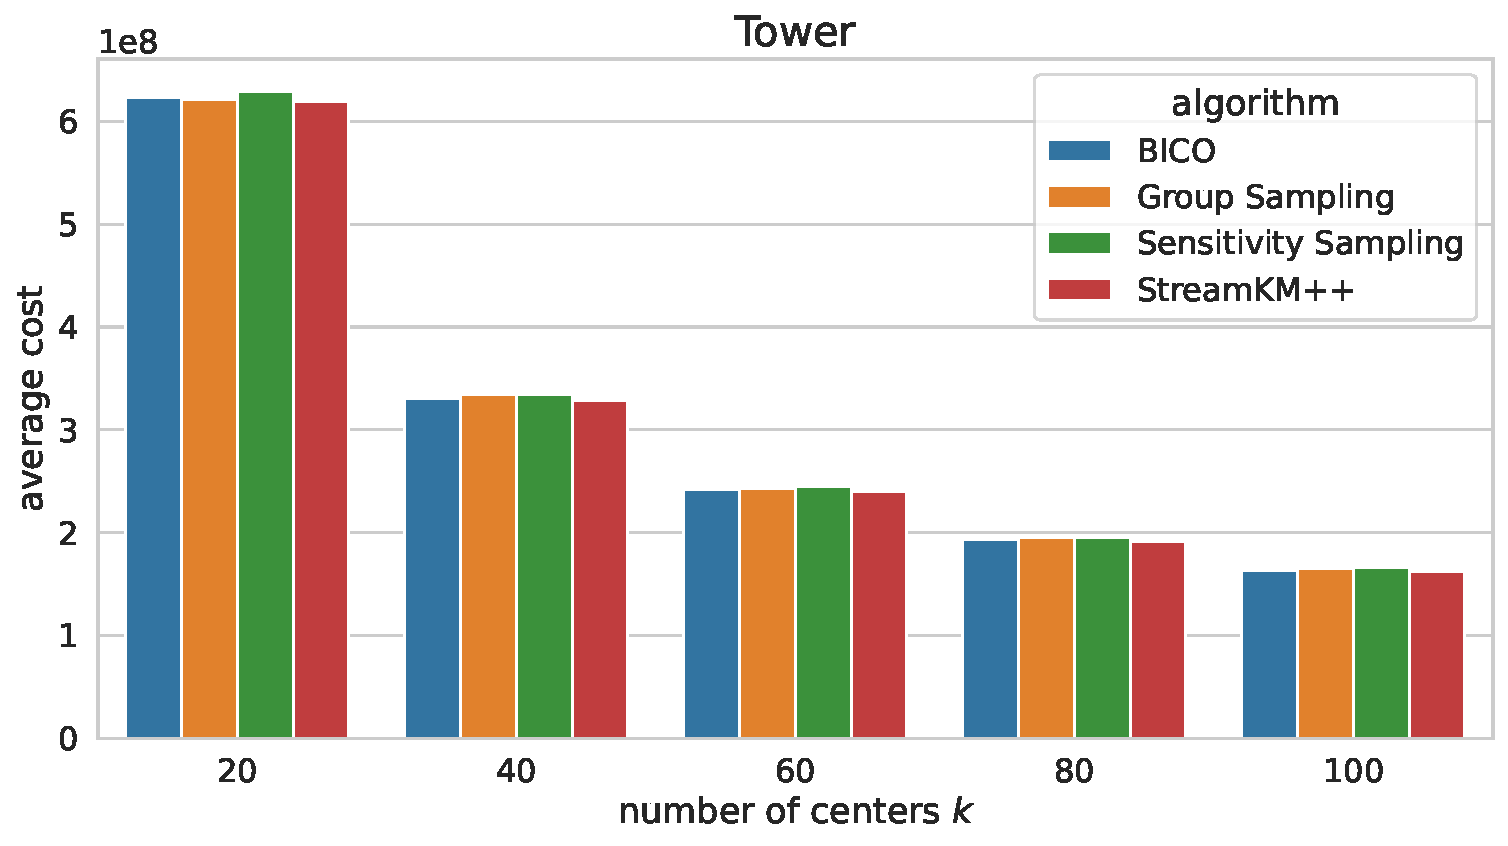
\includegraphics[width=.5\linewidth]{figures/costs-Tower.pdf}
  \newline \newline
  \subfloat{
    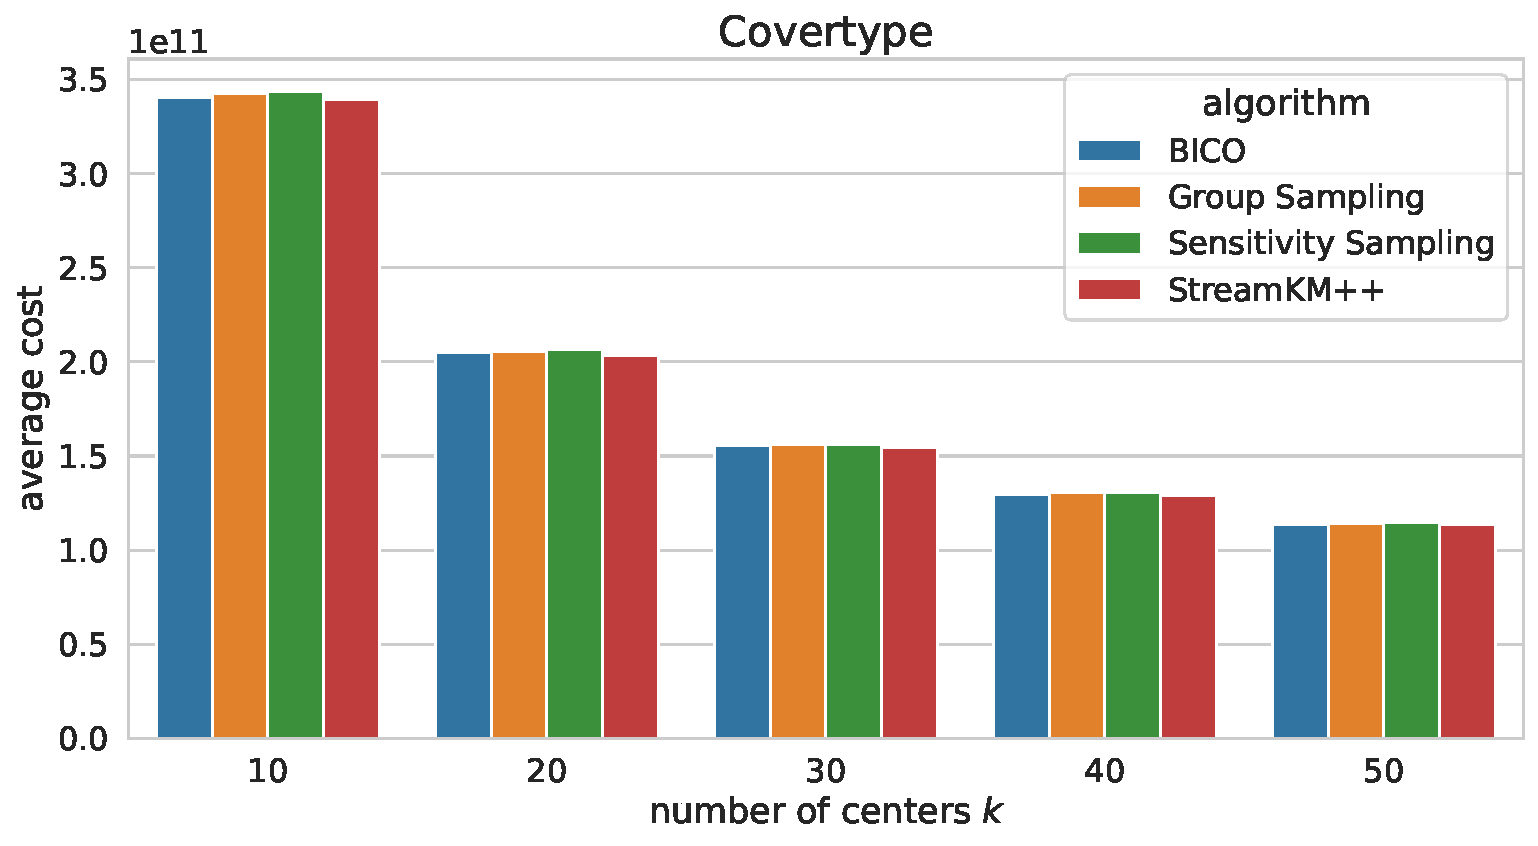
\includegraphics[width=0.5\textwidth]{figures/costs-Covertype.pdf}
  }
  \subfloat{
    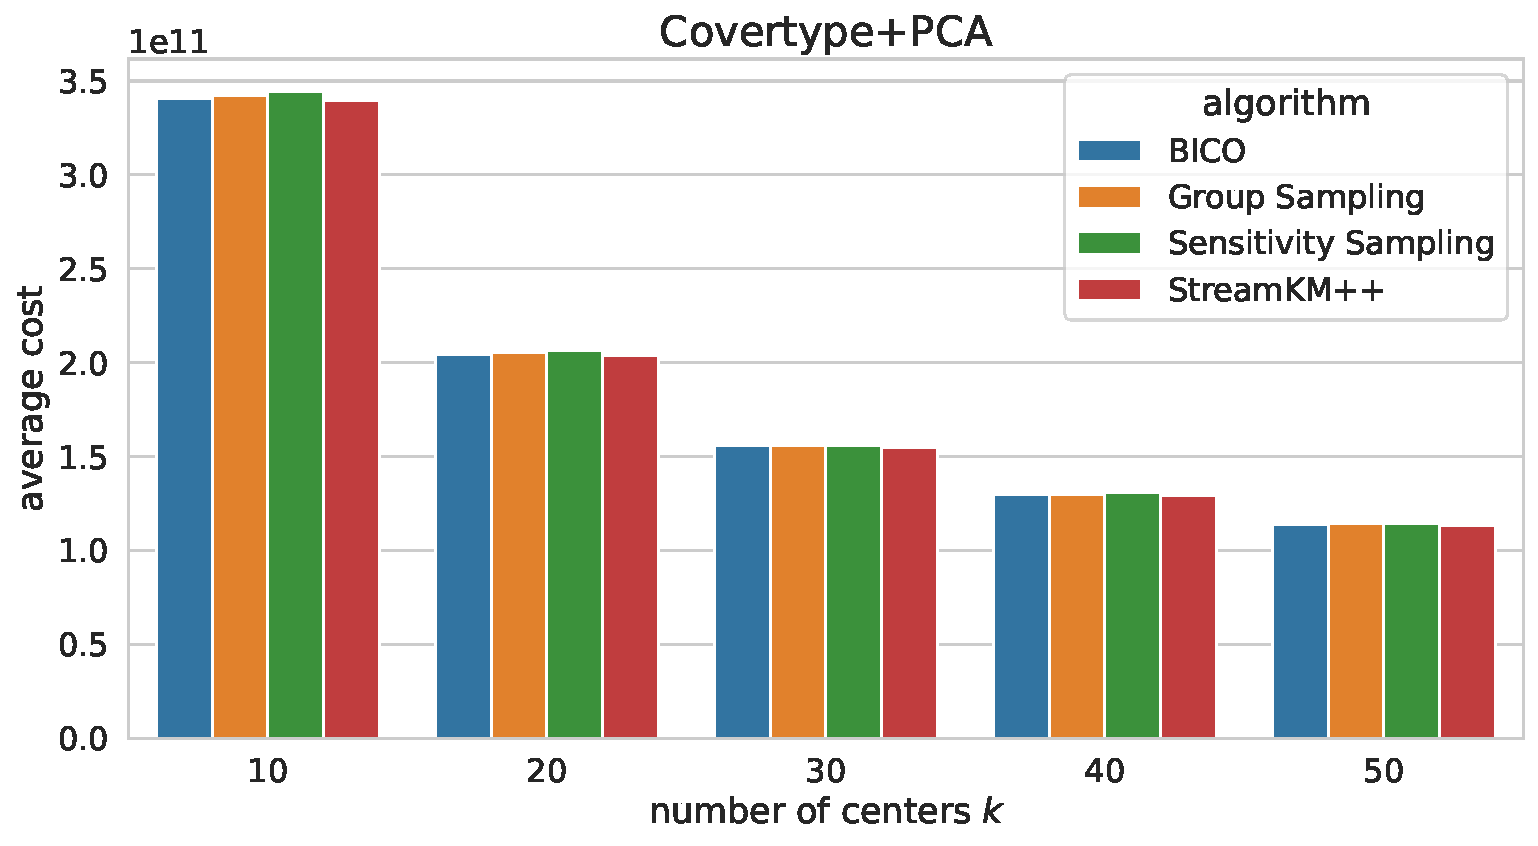
\includegraphics[width=.5\linewidth]{figures/costs-Covertype+PCA.pdf}
  }
  \newline \newline
  \subfloat{
    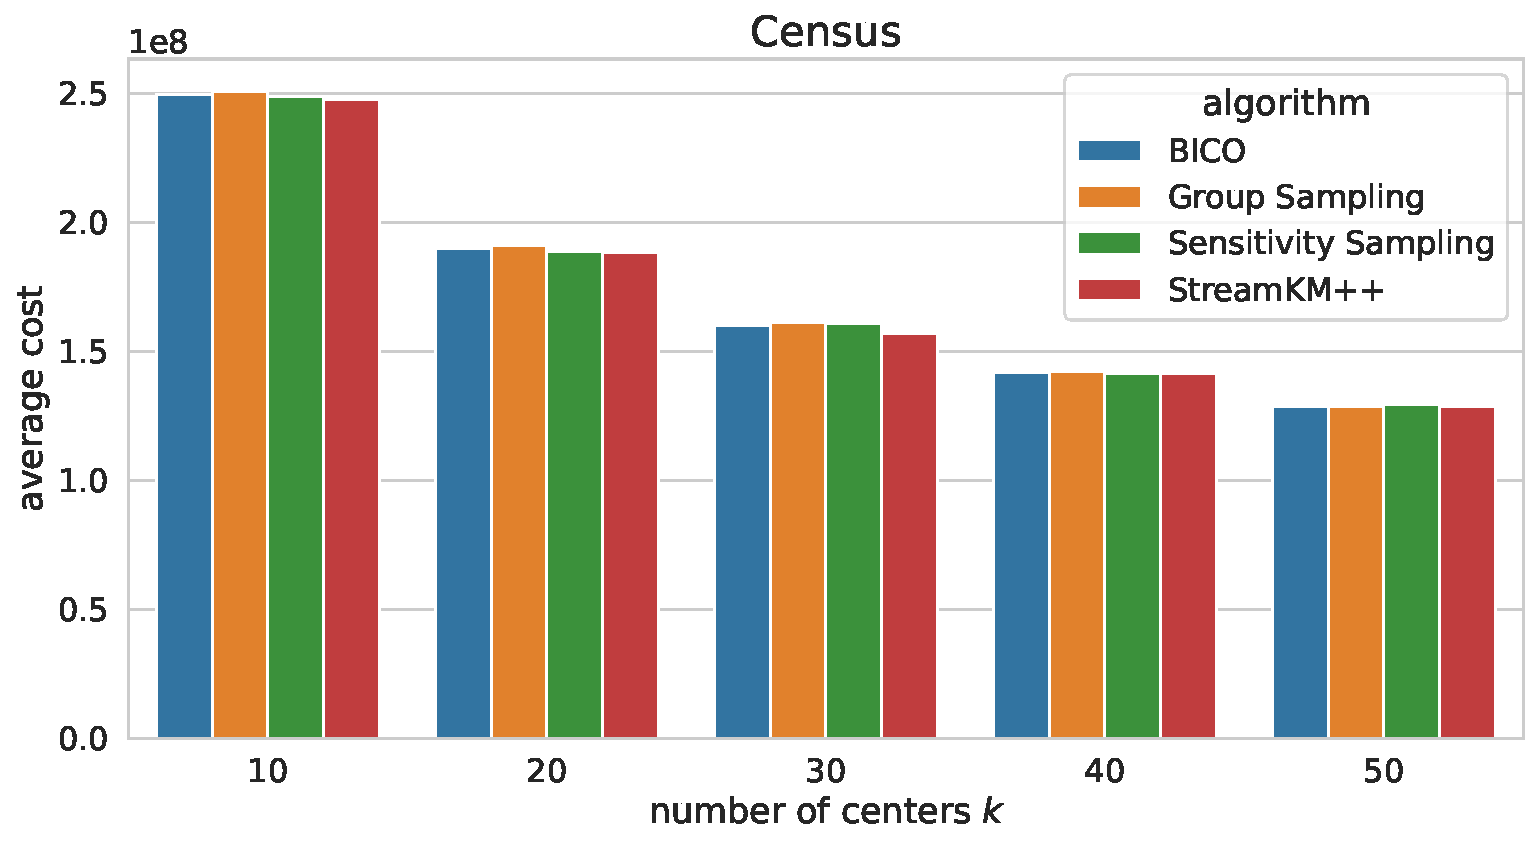
\includegraphics[width=0.5\textwidth]{figures/costs-Census.pdf}
  }
  \subfloat{
    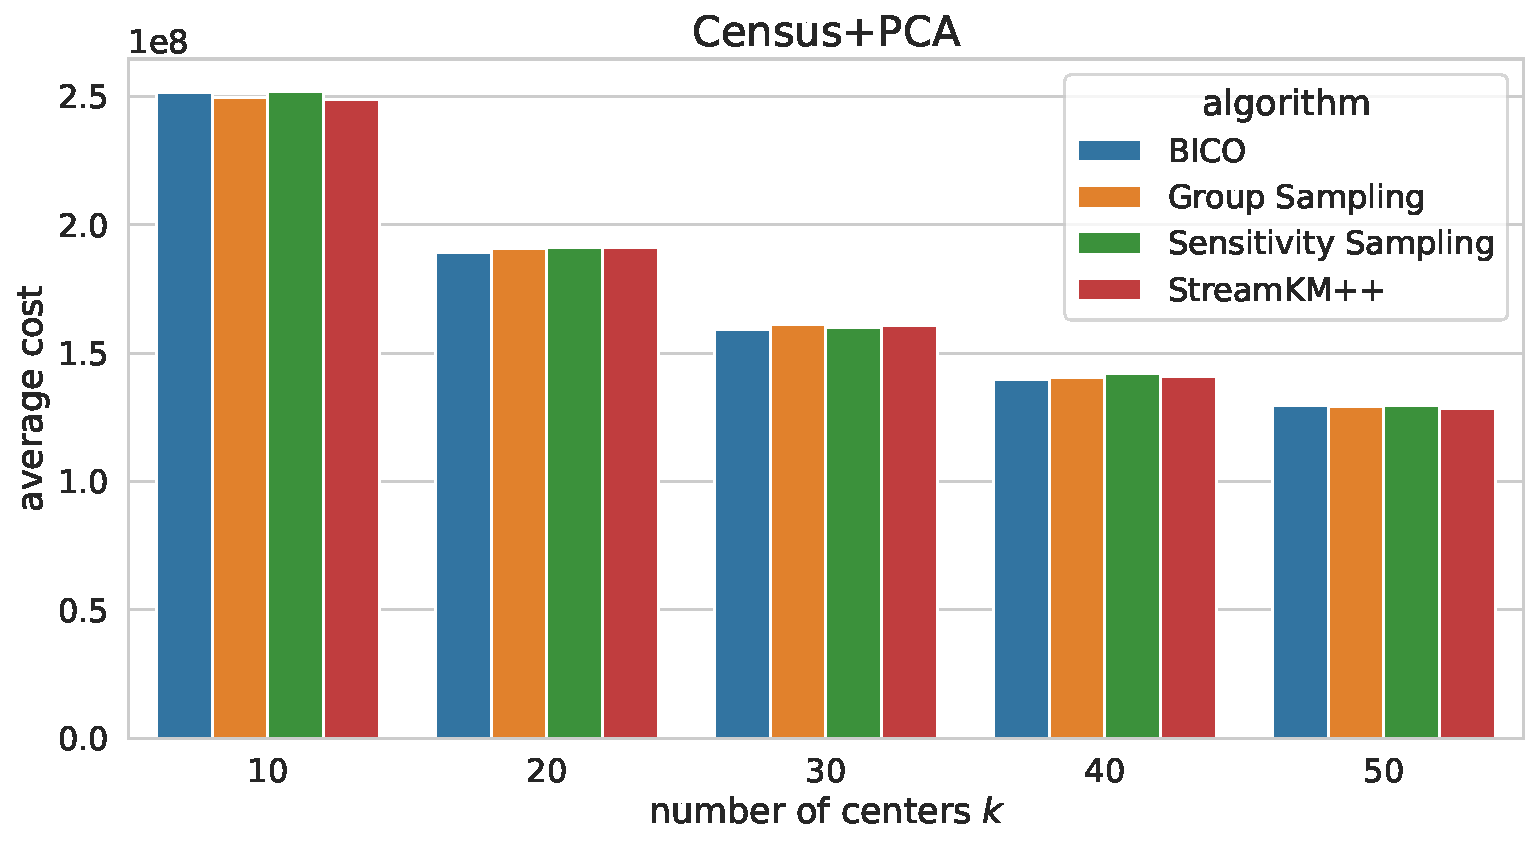
\includegraphics[width=.5\linewidth]{figures/costs-Census+PCA.pdf}
  }
  \newline \newline
  \label{fig:costs}
  \caption{The costs of the evaluated algorithms on \textit{Tower}, \textit{Covertype}, and \textit{Census} datasets.}
\end{figure*}

\section{Conclusion} \label{sec:conclusion}
In this work, we studied how to assess the quality of $k$-means coresets computed by state-of-the-art algorithms. 
Previous work generally measured the quality of optimization algorithms run on the coreset, which we empirically observed to be a poor indicator of coreset quality.
For real data sets, we sampled candidate clusterings and evaluated the worst case distortion on them. Complementing this, we also proposed a benchmark framework which generates hard instances for known $k$-means coreset algorithms. Our experiments indicate a general advantage for algorithms based on importance sampling over movement-based methods aiming towards computing low-cost clusterings.
Despite movement based methods running on very efficient code, it is necessary to complement them with rather expensive dimension reduction methods, rendering what efficiency they might have over importance sampling somewhat moot.

Two results bear further investigation. First, the currently known provable coreset sizes for Sensitivity Sampling are worse than those provable via Group Sampling. Empirically, we observed the opposite: While Group Sampling is competitive, Sensitivity Sampling always outperforms it. Since Group Sampling requires somewhat cumbersome computational overhead, practical applications should prefer Sensitivity Sampling. In light of these results, a theoretical analysis for Sensitivity Sampling matching the performance of Group Sampling would be welcome.

The second point of interest focuses on the performance of StreamKM++. The distortion of this algorithm is significantly better than what one would expect from its theoretical analysis.
Empirically, StreamKM++ is notably better than the other movement-based constructions across all data sets, and especially on high dimensional data.
While it is not competitive to the pure importance sampling algorithms, there are several reasons for investigating it further. It essentially only requires running $k$-means++ for additional iterations, which is already a nearly ubiquitous algorithm for the $k$-means problem. Although the other sampling-based coreset algorithms can also be readily implemented, doing so might be cumbersome. In particular, the theoretically (but not empirically) best algorithm Group Sampling requires extensive preprocessing steps.
This begs the question whether there exist a better theoretical analysis for StreamKM++.

In addition, StreamKM++ currently weighs each point by the number of points assigned to it. It may also be possible to improve the performance of the algorithm in both theory and practice by using a different weighting scheme. 
We leave this as an open problem for future research.

\newpage

\bibliography{references}
\newpage
\appendix
\section{Properties of the Benchmark}

\begin{figure*}[h]
\begin{center}
$$ 
\begin{bmatrix}
\frac{1}{2} & -\frac{1}{2} & \frac{1}{2} & -\frac{1}{2} & \frac{1}{2} & -\frac{1}{2}  \\
-\frac{1}{2} & \frac{1}{2} & \frac{1}{2} & -\frac{1}{2} & \frac{1}{2} & -\frac{1}{2} \\
\frac{1}{2} & -\frac{1}{2} & -\frac{1}{2} & \frac{1}{2} & \frac{1}{2} & -\frac{1}{2}  \\
-\frac{1}{2} & \frac{1}{2} & -\frac{1}{2} & \frac{1}{2} & \frac{1}{2} & -\frac{1}{2} \\
\frac{1}{2} & -\frac{1}{2} & \frac{1}{2} & -\frac{1}{2} & -\frac{1}{2} & \frac{1}{2}  \\
-\frac{1}{2} & \frac{1}{2} & \frac{1}{2} & -\frac{1}{2} & -\frac{1}{2} & \frac{1}{2}  \\
\frac{1}{2} & -\frac{1}{2} & -\frac{1}{2} & \frac{1}{2} &-\frac{1}{2} & \frac{1}{2} \\
-\frac{1}{2} & \frac{1}{2} & -\frac{1}{2} & \frac{1}{2}  & -\frac{1}{2} & \frac{1}{2} \\
\end{bmatrix} ~~~~~~~~
% \begin{bmatrix}
% \frac{2}{3} & -\frac{1}{3} & -\frac{1}{3} & \frac{2}{3} & -\frac{1}{3} & -\frac{1}{3}\\
% \frac{2}{3} & -\frac{1}{3} & -\frac{1}{3} & -\frac{1}{3} & \frac{2}{3} & -\frac{1}{3}\\
% \frac{2}{3} & -\frac{1}{3} & -\frac{1}{3} & -\frac{1}{3} & -\frac{1}{3} & \frac{2}{3}\\
%  -\frac{1}{3} & \frac{2}{3} & -\frac{1}{3} & \frac{2}{3} & -\frac{1}{3} & -\frac{1}{3}\\
% -\frac{1}{3} & \frac{2}{3} & -\frac{1}{3} & -\frac{1}{3} & \frac{2}{3} & -\frac{1}{3}\\
% -\frac{1}{3} & \frac{2}{3} &  -\frac{1}{3} & -\frac{1}{3} & -\frac{1}{3} & \frac{2}{3}\\
% -\frac{1}{3} & -\frac{1}{3} & \frac{2}{3} & \frac{2}{3} & -\frac{1}{3} & -\frac{1}{3}\\
% -\frac{1}{3} & -\frac{1}{3} & \frac{2}{3} & -\frac{1}{3} & \frac{2}{3} & -\frac{1}{3}\\
% -\frac{1}{3} & -\frac{1}{3} & \frac{2}{3} & -\frac{1}{3} & -\frac{1}{3} & \frac{2}{3}\\
% \end{bmatrix} 
\begin{bmatrix}
 \frac{2}{3}   & -\frac{1}{3}  & -\frac{1}{3} & \frac{2}{3}   & -\frac{1}{3}  & -\frac{1}{3}   \\
 -\frac{1}{3}  & \frac{2}{3}   & -\frac{1}{3} & \frac{2}{3}   & -\frac{1}{3}  & -\frac{1}{3}   \\
 -\frac{1}{3}  & -\frac{1}{3}  & \frac{2}{3}  & \frac{2}{3}   & -\frac{1}{3}  & -\frac{1}{3}   \\
 \frac{2}{3}   & -\frac{1}{3}  & -\frac{1}{3} & -\frac{1}{3}  & \frac{2}{3}   & -\frac{1}{3}   \\
 -\frac{1}{3}  & \frac{2}{3}   & -\frac{1}{3} & -\frac{1}{3}  & \frac{2}{3}   & -\frac{1}{3}   \\
 -\frac{1}{3}  & -\frac{1}{3}  & \frac{2}{3}  & -\frac{1}{3}  & \frac{2}{3}   &  -\frac{1}{3}  \\
 \frac{2}{3}   & -\frac{1}{3}  & -\frac{1}{3} & -\frac{1}{3}  & -\frac{1}{3}  & \frac{2}{3}    \\
 -\frac{1}{3}  & \frac{2}{3}   & -\frac{1}{3} & -\frac{1}{3}  & -\frac{1}{3}  & \frac{2}{3}    \\
 -\frac{1}{3}  & -\frac{1}{3}  & \frac{2}{3}  & -\frac{1}{3}  & -\frac{1}{3}  & \frac{2}{3}    \\
\end{bmatrix} 
$$
\end{center}
\caption{Benchmark construction for $k=2$ and $\alpha=3$ (left) and $k=3$ and $\alpha=2$ (right).}
\label{fig:benchmark-small-instances}
\end{figure*}


\begin{fact}
For $a\neq a'$, we have $d(\mathcal{C}^{a},\mathcal{C}^{a'}) = 1-1/k$.
\end{fact}
\begin{proof}
Consider an arbitrary vector $v_i^{\ell}$. By construction, the positive entries of $v_i^{\ell}$ range from $k^{\ell-1}\cdot i+1$ to $k^{\ell-1}\cdot (i+1)$. Similarly, the positive entries for the vector $v_j^{\ell-1}$ range from range from $k^{\ell-2}\cdot j+1$ to $k^{\ell-2}\cdot (j+1)$. Therefore, concatenating $v_j^{\ell-1}$ $k$ times into a vector $v'$, $v'$ and $v_i^{\ell}$ can share at most one positive coordinate. Inductively, the same holds true for any concatenation of vectors $v_j^{\ell-h}$.
Thus, the two clusters induced by the columns formed by concatenating the vectors $v$ can share only a $1/k$ fraction of the points. Since each cluster consists of exactly $k^{\alpha}/k$ = $k^{\alpha-1}$ points, the confusion matrix $M$ only has entries $\frac{n}{k^2}$ and for any permutation $\pi$, we have $d(\mathcal{C}^{a},\mathcal{C}^{a'}) = 1-1/k$.
\end{proof}

\begin{fact}
\label{fact:cost}
For any $C_j^a$, we have $\cost_{C_j^a}(\{\mu(C_j^a)\}) = (\alpha-1)\cdot k^{\alpha-2}\cdot (k-1)$.
\end{fact}
\begin{proof}
Without loss of generality, we consider $C_1^0$; the proof is analogous for the other choices of $j$ and $a$. We first note that for any point $A_i \in C_1^0$, the coordinates $A_{i,\ell}$ are identical for $\ell <k$. Furthermore for the column $\ell\geq k$, we have by construction $\sum_{A_i\in C_j} A_{i,\ell} = k^{\alpha-1}\cdot \frac{k-1}{k} + (k^{\alpha}-k^{\alpha-1})\frac{1}{k}=k^{\alpha-1}\cdot (\frac{k-1}{k} - (k-1)\frac{1}{k}) = 0.$ Therefore, the mean of $C_1^0$ satisfies $\mu(C_1^0)_{\ell} = \begin{cases}A_{i,\ell} &\text{if }\ell<k \\
0 &\text{else.}\end{cases}$. 
Thus, the cost is precisely $(\alpha-1)\cdot k^{\alpha-1}\cdot \left(\left(\frac{k-1}{k}\right)^2 + \left(\frac{1}{k}\right)^2 \right)=(\alpha-1)\cdot k^{\alpha-2}\cdot (k-1)$.
\end{proof}

Finally, we show that the means for the clustering $\mathcal{C}^{a}$ also induce $\mathcal{C}^{a}$.

\begin{fact}
\label{fact:opt}
For a clustering $\mathcal{C}^{a}$, let $\mu(C_j^{a})$ denote the mean of cluster $C_j^a$. Then every point  is assigned to its closest center. Moreover, every point $A_i$ of $C_j^a$ has equal distance to any center $\mu(C_h^{a})$ with $h\neq j$.
\end{fact}
\begin{proof}
Again, we assume without loss of generality $a=0$.
Let $A_i$ be an arbitrary point of cluster $C_{h}^{a}$ and consider the mean $\mu(C_j^a)_{\ell} = \begin{cases}A_{i,\ell} &\text{if }\ell<k \\
0 &\text{else.}\end{cases}$ of cluster $C_j^a$. By definition, the positive coordinates of $A_i$ are not equal to the positive coordinates of $\mu(C_j^a)$. The only difference in coordinates between the means of $\mu(C_j^a)$ and $\mu(C_h^a)$ are the first $k$ coordinates, as the rest are $0$.
But here the coordinates of $\mu(C_h^a)$ and $A_i$ are identical, hence $\mu(C_j^a)$ cannot be closer to $A_i$.

To prove that the distances between $A_i$ and any $\mu(C_h^{a})$ with $h\neq j$ are equal, again consider that any difference can only exist among the first $k$ coordinates. Here, we have $\mu(C_h^{a})_h = \frac{k-1}{k}$, and the remaining columns are $-\frac{1}{k}$. Since $A_{i,h} = -\frac{1}{k}$ for any $h\neq j$, the claim follows.
\end{proof}

\section{Hardness of Weak Coreset Evaluation}

Here, we show that it is in general co-NP hard to evaluate whether two point sets $A$ and $B$ are weak coresets of each other. A weak coreset only requires that a $(1+\varepsilon)$ approximation for one point set is a $(1+O(\varepsilon))$ for the other.


\begin{proposition}
\label{prop:hardness}
Given two point sets $A$ and $B$ in $\mathbb{R}^d$ and a sufficiently small (constant) $\varepsilon>0$, it is co-NP hard to decide whether $A$ is a weak coreset of $B$.
\end{proposition}
\begin{proof}
First, we recall that for some $\varepsilon_0$ and candidate clustering cost $V$, it is NP-hard to decide whether there exists a clustering $C$ with cost in $\cost_A(C)\leq V$ and $\cost_B(C)\geq (1+\varepsilon_0)\cdot V$.
Conversely, it is co-NP-hard to decide whether there exists no set of centers $C$ such that $\cost_A(C)\leq V$ and $\cost_B(C) \geq (1+\varepsilon_0)\cdot V$.
\end{proof}

We remark that the possible values for $\varepsilon_0$ are determined by the current APX-hardness results. Assuming NP$\neq$P, $\varepsilon_0\approx 1.07$ and assuming UCG, $\varepsilon_0 \approx 1.17$~\cite{Cohen-AddadSL21,Cohen-AddadS19} for $k$-means in Euclidean spaces.




\section{Distortions}


The tables 
(\cref{tab:distortions-mean-std-benchmark},
 \cref{tab:distortions-mean-std-caltech},
 \cref{tab:distortions-mean-std-caltech-pca},
 \cref{tab:distortions-mean-std-census},
 \cref{tab:distortions-mean-std-census-pca},
 \cref{tab:distortions-mean-std-covertype},
 \cref{tab:distortions-mean-std-covertype-pca},
 \cref{tab:distortions-mean-std-nytimes},
 \cref{tab:distortions-mean-std-nytimes-pca},
 \cref{tab:distortions-mean-std-tower})
show the distortions of the 5 evaluated algorithms on the different data sets.
We vary the coreset size $T$ for different $k$ values using the formula: $T=mk$ where $m = \{50, 100, 200, 500\}$.
The running time for StreamKM++ with coreset size $T=500k$ exceeds the allocated time budget of 32 hours on almost all data sets.
For this reason, the distortions for StreamKM++ with $m=500$ are not present in the tables.



\begin{longtable}{lllllll}
\multicolumn{7}{c}{\textbf{Distortions on the \textit{Caltech} data set}} \\
\toprule
\parbox[t]{5mm}{\ \\$k$} 
& \parbox[t]{5mm}{\ \\$m$} 
& BICO 
& \parbox[t]{1.7cm}{Group\\Sampling} 
& \parbox[t]{1.7cm}{Ray\\Maker}
& \parbox[t]{1.7cm}{Sensitivity\\Sampling}
&    StreamKM++ \\
\midrule
10 & 50  &  3.40 (0.440) &   1.02 (0.010) &  5.05 (0.157) &         1.02 (0.005) &  1.07 (0.005) \\
   & 100 &  3.24 (0.729) &   1.01 (0.004) &  3.84 (0.081) &         1.01 (0.003) &  1.05 (0.004) \\
   & 200 &  2.90 (0.153) &   1.01 (0.002) &  3.48 (0.052) &         1.01 (0.002) &  1.04 (0.002) \\
   & 500 &  2.62 (0.095) &   1.01 (0.001) &  3.40 (0.058) &         1.00 (0.001) &  \\
 \midrule
20 & 50  &  3.22 (0.160) &   1.04 (0.004) &  5.52 (0.266) &         1.02 (0.003) &  1.08 (0.006) \\
   & 100 &  3.09 (0.122) &   1.02 (0.004) &  4.31 (0.130) &         1.01 (0.002) &  1.08 (0.003) \\
   & 200 &  2.88 (0.078) &   1.01 (0.002) &  3.93 (0.120) &         1.01 (0.001) &  1.11 (0.002) \\
   & 500 &  2.36 (0.051) &   1.01 (0.001) &  3.81 (0.116) &         1.01 (0.001) &  \\
 \midrule
30 & 50  &  2.81 (0.244) &   1.03 (0.006) &  6.43 (0.470) &         1.02 (0.002) &  1.13 (0.004) \\
   & 100 &  2.58 (0.105) &   1.02 (0.003) &  4.65 (0.256) &         1.02 (0.002) &  1.13 (0.004) \\
   & 200 &  2.38 (0.098) &   1.01 (0.002) &  4.12 (0.234) &         1.01 (0.002) &  1.10 (0.002) \\
   & 500 &  2.01 (0.065) &   1.01 (0.001) &  4.00 (0.138) &         1.01 (0.001) &  \\
 \midrule
40 & 50  &  3.16 (0.500) &   1.03 (0.004) &  5.62 (0.287) &         1.02 (0.004) &  1.10 (0.004) \\
   & 100 &  2.78 (0.258) &   1.02 (0.001) &  4.42 (0.200) &         1.02 (0.002) &  1.14 (0.003) \\
   & 200 &  2.79 (0.217) &   1.02 (0.001) &  3.82 (0.111) &         1.01 (0.001) &  1.17 (0.004) \\
   & 500 &  2.57 (0.113) &   1.01 (0.001) &  3.86 (0.122) &         1.01 (0.001) &            \\
\bottomrule
\caption{Distortions of the evaluated algorithms on the \textit{Benchmark} data set. Each cell specify the mean distortion along with the standard deviation in parenthesis of 10 repetitions of the experiment.}
\label{tab:distortions-mean-std-benchmark}
\end{longtable}

\begin{longtable}{lllllll}
\multicolumn{7}{c}{\textbf{Distortions on the \textit{Caltech} data set}} \\
\toprule
\parbox[t]{5mm}{\ \\$k$} 
& \parbox[t]{5mm}{\ \\$m$} 
& BICO 
& \parbox[t]{1.7cm}{Group\\Sampling} 
& \parbox[t]{1.7cm}{Ray\\Maker}
& \parbox[t]{1.7cm}{Sensitivity\\Sampling}
&    StreamKM++ \\
\midrule
10 & 50  &  5.12 (0.307) &   1.07 (0.009) &  7.05 (0.250) &         1.05 (0.013) &  1.16 (0.008) \\
   & 100 &  4.48 (0.284) &   1.04 (0.006) &  5.46 (0.254) &         1.03 (0.008) &  1.13 (0.005) \\
   & 200 &  4.08 (0.319) &   1.02 (0.004) &  5.00 (0.196) &         1.01 (0.005) &  1.10 (0.005) \\
   & 500 &  3.41 (0.215) &   1.01 (0.003) &  4.75 (0.188) &         1.00 (0.003) &  \\
 \midrule
20 & 50  &  6.35 (1.173) &   1.06 (0.008) &  6.92 (0.209) &         1.05 (0.007) &  1.18 (0.008) \\
   & 100 &  4.65 (0.283) &   1.04 (0.005) &  5.29 (0.146) &         1.03 (0.005) &  1.14 (0.005) \\
   & 200 &  4.19 (0.384) &   1.02 (0.002) &  4.80 (0.112) &         1.01 (0.004) &  1.12 (0.004) \\
   & 500 &  3.50 (0.404) &   1.01 (0.002) &  4.61 (0.096) &         1.00 (0.001) &  \\
 \midrule
30 & 50  &  6.01 (0.335) &   1.06 (0.005) &  6.79 (0.149) &         1.04 (0.004) &  1.19 (0.005) \\
   & 100 &  5.10 (0.628) &   1.04 (0.005) &  5.30 (0.123) &         1.02 (0.005) &  1.15 (0.002) \\
   & 200 &  4.29 (0.659) &   1.02 (0.003) &  4.70 (0.075) &         1.01 (0.003) &  1.13 (0.002) \\
   & 500 &  3.09 (0.138) &   1.01 (0.002) &  4.62 (0.090) &         1.00 (0.002) &  \\
 \midrule
40 & 50  &  6.24 (0.524) &   1.07 (0.004) &  6.85 (0.145) &         1.05 (0.004) &  1.20 (0.004) \\
   & 100 &  5.23 (0.874) &   1.04 (0.003) &  5.22 (0.092) &         1.02 (0.002) &  1.16 (0.003) \\
   & 200 &  4.50 (1.085) &   1.02 (0.002) &  4.72 (0.086) &         1.01 (0.001) &  1.13 (0.002) \\
   & 500 &  3.38 (0.398) &   1.01 (0.001) &  4.55 (0.094) &         1.00 (0.001) &  \\
 \midrule
50 & 50  &  7.50 (1.013) &   1.07 (0.004) &  6.80 (0.092) &         1.05 (0.004) &  1.20 (0.006) \\
   & 100 &  5.21 (0.968) &   1.04 (0.003) &  5.18 (0.084) &         1.03 (0.002) &  1.16 (0.005) \\
   & 200 &  4.21 (0.296) &   1.02 (0.002) &  4.69 (0.065) &         1.01 (0.003) &  1.13 (0.002) \\
   & 500 &  3.36 (0.429) &   1.01 (0.001) &  4.52 (0.058) &         1.00 (0.001) &            \\
\bottomrule
\caption{Distortions of the evaluated algorithms on the \textit{Caltech} data set. Each cell specify the mean distortion along with the standard deviation in parenthesis of 10 repetitions of the experiment.}
\label{tab:distortions-mean-std-caltech}
\end{longtable}

\begin{longtable}{lllllll}
\multicolumn{7}{c}{\textbf{Distortions on the \textit{Caltech} data set (with PCA preprocessing)}} \\
\toprule
\parbox[t]{5mm}{\ \\$k$} & \parbox[t]{5mm}{\ \\$m$} &BICO & \parbox[t]{1.7cm}{Group\\Sampling} &\parbox[t]{1.7cm}{Ray\\Maker}&\parbox[t]{1.7cm}{Sensitivity\\Sampling}&    StreamKM++ \\
\midrule
10 & 50  &  1.21 (0.009) &   1.03 (0.004) &  1.25 (0.005) &         1.02 (0.007) &  1.04 (0.005) \\
   & 100 &  1.19 (0.006) &   1.02 (0.006) &  1.21 (0.006) &         1.01 (0.004) &  1.03 (0.004) \\
   & 200 &  1.16 (0.003) &   1.01 (0.002) &  1.19 (0.003) &         1.01 (0.003) &  1.02 (0.002) \\
   & 500 &  1.13 (0.007) &   1.00 (0.002) &  1.19 (0.006) &         1.00 (0.001) &  \\
 \midrule
20 & 50  &  1.54 (0.024) &   1.04 (0.006) &  1.63 (0.008) &         1.03 (0.006) &  1.07 (0.003) \\
   & 100 &  1.48 (0.020) &   1.02 (0.002) &  1.54 (0.010) &         1.01 (0.004) &  1.06 (0.003) \\
   & 200 &  1.41 (0.006) &   1.01 (0.002) &  1.50 (0.011) &         1.01 (0.003) &  1.04 (0.003) \\
   & 500 &  1.35 (0.008) &   1.00 (0.001) &  1.49 (0.008) &         1.00 (0.001) &  \\
 \midrule
30 & 50  &  1.99 (0.032) &   1.05 (0.006) &  2.05 (0.020) &         1.03 (0.003) &  1.10 (0.004) \\
   & 100 &  1.82 (0.099) &   1.03 (0.004) &  1.90 (0.014) &         1.02 (0.003) &  1.08 (0.002) \\
   & 200 &  1.72 (0.046) &   1.01 (0.002) &  1.84 (0.009) &         1.01 (0.002) &  1.06 (0.002) \\
   & 500 &  1.62 (0.037) &   1.01 (0.001) &  1.81 (0.011) &         1.00 (0.002) &  \\
 \midrule
40 & 50  &  2.34 (0.112) &   1.05 (0.003) &  2.48 (0.020) &         1.04 (0.005) &  1.12 (0.004) \\
   & 100 &  2.25 (0.066) &   1.03 (0.003) &  2.23 (0.011) &         1.02 (0.001) &  1.09 (0.003) \\
   & 200 &  2.11 (0.072) &   1.02 (0.002) &  2.15 (0.012) &         1.01 (0.003) &  1.07 (0.002) \\
   & 500 &  1.90 (0.070) &   1.01 (0.002) &  2.12 (0.011) &         1.00 (0.001) &  \\
 \midrule
50 & 50  &  2.86 (0.214) &   1.06 (0.003) &  2.94 (0.026) &         1.04 (0.005) &  1.14 (0.005) \\
   & 100 &  2.58 (0.124) &   1.03 (0.001) &  2.59 (0.019) &         1.02 (0.001) &  1.11 (0.002) \\
   & 200 &  2.35 (0.139) &   1.02 (0.001) &  2.49 (0.021) &         1.01 (0.002) &  1.09 (0.002) \\
   & 500 &  2.15 (0.075) &   1.01 (0.001) &  2.44 (0.015) &         1.00 (0.001) &            \\
\bottomrule
\caption{Distortions of the evaluated algorithms on the \textit{Caltech} data set (with PCA preprocessing). Each cell specify the mean distortion along with the standard deviation in parenthesis of 10 repetitions of the experiment.}
\label{tab:distortions-mean-std-caltech-pca}
\end{longtable}

\begin{longtable}{lllllll}
\multicolumn{7}{c}{\textbf{Distortions on the \textit{Census} data set}} \\
\toprule
\parbox[t]{5mm}{\ \\$k$} & \parbox[t]{5mm}{\ \\$m$} &BICO & \parbox[t]{1.7cm}{Group\\Sampling} &\parbox[t]{1.7cm}{Ray\\Maker}&\parbox[t]{1.7cm}{Sensitivity\\Sampling}&    StreamKM++ \\
\midrule
10 & 50  &  2.08 (0.106) &   1.08 (0.019) &  2.30 (0.162) &         1.03 (0.031) &  1.10 (0.012) \\
   & 100 &  1.83 (0.124) &   1.04 (0.021) &  1.92 (0.094) &         1.03 (0.012) &  1.07 (0.006) \\
   & 200 &  1.65 (0.056) &   1.02 (0.005) &  1.72 (0.050) &         1.02 (0.012) &  1.05 (0.005) \\
   & 500 &  1.48 (0.053) &   1.02 (0.004) &  1.69 (0.029) &         1.02 (0.010) &  \\
 \midrule
20 & 50  &  2.18 (0.164) &   1.07 (0.022) &  2.31 (0.078) &         1.03 (0.007) &  1.10 (0.008) \\
   & 100 &  1.93 (0.080) &   1.04 (0.011) &  1.91 (0.048) &         1.02 (0.011) &  1.08 (0.005) \\
   & 200 &  1.71 (0.031) &   1.03 (0.006) &  1.75 (0.027) &         1.01 (0.006) &  1.06 (0.004) \\
   & 500 &  1.51 (0.048) &   1.02 (0.005) &  1.66 (0.019) &         1.01 (0.004) &  \\
 \midrule
30 & 50  &  2.28 (0.177) &   1.07 (0.011) &  2.38 (0.077) &         1.03 (0.011) &  1.11 (0.007) \\
   & 100 &  2.05 (0.096) &   1.04 (0.006) &  1.95 (0.040) &         1.02 (0.007) &  1.09 (0.004) \\
   & 200 &  1.76 (0.055) &   1.03 (0.005) &  1.79 (0.034) &         1.01 (0.007) &  1.07 (0.003) \\
   & 500 &  1.56 (0.016) &   1.01 (0.003) &  1.71 (0.038) &         1.01 (0.003) &  \\
 \midrule
40 & 50  &  2.47 (0.101) &   1.08 (0.009) &  2.43 (0.069) &         1.02 (0.010) &  1.12 (0.006) \\
   & 100 &  2.11 (0.104) &   1.04 (0.006) &  1.99 (0.034) &         1.01 (0.004) &  1.09 (0.003) \\
   & 200 &  1.83 (0.038) &   1.02 (0.007) &  1.81 (0.026) &         1.01 (0.005) &  1.08 (0.002) \\
   & 500 &  1.56 (0.039) &   1.01 (0.005) &  1.73 (0.026) &         1.01 (0.003) &  \\
 \midrule
50 & 50  &  2.50 (0.138) &   1.07 (0.008) &  2.48 (0.054) &         1.02 (0.011) &  1.13 (0.004) \\
   & 100 &  2.12 (0.109) &   1.04 (0.007) &  2.02 (0.055) &         1.01 (0.004) &  1.10 (0.003) \\
   & 200 &  1.84 (0.059) &   1.03 (0.004) &  1.82 (0.022) &         1.01 (0.005) &  1.08 (0.004) \\
   & 500 &  1.57 (0.019) &   1.02 (0.004) &  1.75 (0.022) &         1.01 (0.003) &            \\
\bottomrule
\caption{Distortions of the evaluated algorithms on the \textit{Census} data set. Each cell specify the mean distortion along with the standard deviation in parenthesis of 10 repetitions of the experiment.}
\label{tab:distortions-mean-std-census}
\end{longtable}

\begin{longtable}{lllllll}
\multicolumn{7}{c}{\textbf{Distortions on the \textit{Census} data set (with PCA preprocessing)}} \\
\toprule
\parbox[t]{5mm}{\ \\$k$} & \parbox[t]{5mm}{\ \\$m$} &BICO & \parbox[t]{1.7cm}{Group\\Sampling} &\parbox[t]{1.7cm}{Ray\\Maker}&\parbox[t]{1.7cm}{Sensitivity\\Sampling}&    StreamKM++ \\
\midrule
10 & 50  &  1.34 (0.048) &   1.06 (0.018) &  1.35 (0.030) &         1.04 (0.021) &  1.03 (0.007) \\
   & 100 &  1.24 (0.015) &   1.03 (0.007) &  1.25 (0.017) &         1.03 (0.016) &  1.02 (0.005) \\
   & 200 &  1.19 (0.020) &   1.02 (0.009) &  1.19 (0.013) &         1.02 (0.018) &  1.01 (0.002) \\
   & 500 &  1.11 (0.003) &   1.01 (0.005) &  1.18 (0.017) &         1.01 (0.003) &  \\
 \midrule
20 & 50  &  1.84 (0.118) &   1.07 (0.018) &  1.78 (0.052) &         1.02 (0.012) &  1.07 (0.005) \\
   & 100 &  1.57 (0.073) &   1.03 (0.010) &  1.56 (0.020) &         1.02 (0.008) &  1.05 (0.005) \\
   & 200 &  1.44 (0.037) &   1.02 (0.007) &  1.44 (0.030) &         1.01 (0.008) &  1.03 (0.002) \\
   & 500 &  1.30 (0.014) &   1.01 (0.005) &  1.39 (0.017) &         1.01 (0.005) &  \\
 \midrule
30 & 50  &  2.13 (0.153) &   1.07 (0.010) &  2.10 (0.045) &         1.02 (0.011) &  1.10 (0.005) \\
   & 100 &  1.81 (0.050) &   1.04 (0.009) &  1.79 (0.029) &         1.01 (0.006) &  1.07 (0.003) \\
   & 200 &  1.63 (0.044) &   1.02 (0.006) &  1.65 (0.029) &         1.01 (0.005) &  1.06 (0.002) \\
   & 500 &  1.47 (0.021) &   1.01 (0.004) &  1.58 (0.014) &         1.01 (0.004) &  \\
 \midrule
40 & 50  &  2.37 (0.102) &   1.07 (0.007) &  2.31 (0.039) &         1.03 (0.008) &  1.11 (0.006) \\
   & 100 &  2.01 (0.118) &   1.04 (0.007) &  1.90 (0.027) &         1.01 (0.004) &  1.09 (0.004) \\
   & 200 &  1.76 (0.027) &   1.03 (0.005) &  1.75 (0.024) &         1.01 (0.002) &  1.07 (0.002) \\
   & 500 &  1.52 (0.044) &   1.02 (0.003) &  1.67 (0.022) &         1.01 (0.003) &  \\
 \midrule
50 & 50  &  2.45 (0.139) &   1.07 (0.008) &  2.46 (0.048) &         1.02 (0.012) &  1.13 (0.004) \\
   & 100 &  2.14 (0.135) &   1.04 (0.007) &  1.99 (0.028) &         1.01 (0.004) &  1.10 (0.003) \\
   & 200 &  1.87 (0.055) &   1.03 (0.005) &  1.82 (0.018) &         1.01 (0.004) &  1.08 (0.002) \\
   & 500 &  1.56 (0.008) &   1.02 (0.004) &  1.73 (0.036) &         1.01 (0.004) &            \\
\bottomrule
\caption{Distortions of the evaluated algorithms on the \textit{Census} data set (with PCA preprocessing). Each cell specify the mean distortion along with the standard deviation in parenthesis of 10 repetitions of the experiment.}
\label{tab:distortions-mean-std-census-pca}
\end{longtable}

\begin{longtable}{lllllll}
\multicolumn{7}{c}{\textbf{Distortions on the \textit{Covertype} data set}} \\
\toprule
\parbox[t]{5mm}{\ \\$k$} & \parbox[t]{5mm}{\ \\$m$} &BICO & \parbox[t]{1.7cm}{Group\\Sampling} &\parbox[t]{1.7cm}{Ray\\Maker}&\parbox[t]{1.7cm}{Sensitivity\\Sampling}&    StreamKM++ \\
\midrule
10 & 50  &  1.25 (0.018) &   1.08 (0.022) &  1.31 (0.027) &         1.04 (0.025) &  1.05 (0.008) \\
   & 100 &  1.17 (0.015) &   1.04 (0.016) &  1.22 (0.017) &         1.03 (0.014) &  1.02 (0.003) \\
   & 200 &  1.11 (0.004) &   1.03 (0.012) &  1.18 (0.014) &         1.02 (0.008) &  1.02 (0.002) \\
   & 500 &  1.05 (0.001) &   1.01 (0.004) &  1.16 (0.009) &         1.01 (0.006) &  \\
 \midrule
20 & 50  &  1.27 (0.025) &   1.09 (0.022) &  1.35 (0.031) &         1.04 (0.008) &  1.05 (0.006) \\
   & 100 &  1.18 (0.004) &   1.05 (0.016) &  1.24 (0.010) &         1.02 (0.006) &  1.03 (0.003) \\
   & 200 &  1.11 (0.003) &   1.02 (0.008) &  1.21 (0.017) &         1.01 (0.007) &  1.01 (0.002) \\
   & 500 &  1.04 (0.001) &   1.01 (0.004) &  1.19 (0.009) &         1.01 (0.006) &  \\
 \midrule
30 & 50  &  1.29 (0.008) &   1.08 (0.017) &  1.37 (0.013) &         1.04 (0.013) &  1.05 (0.005) \\
   & 100 &  1.17 (0.003) &   1.05 (0.007) &  1.26 (0.013) &         1.01 (0.007) &  1.03 (0.003) \\
   & 200 &  1.10 (0.001) &   1.03 (0.009) &  1.21 (0.008) &         1.01 (0.005) &  1.01 (0.001) \\
   & 500 &  1.04 (0.000) &   1.01 (0.003) &  1.20 (0.006) &         1.01 (0.003) &  \\
 \midrule
40 & 50  &  1.28 (0.009) &   1.09 (0.014) &  1.39 (0.012) &         1.03 (0.013) &  1.05 (0.004) \\
   & 100 &  1.18 (0.005) &   1.05 (0.011) &  1.26 (0.009) &         1.02 (0.007) &  1.03 (0.002) \\
   & 200 &  1.09 (0.002) &   1.02 (0.003) &  1.22 (0.008) &         1.01 (0.005) &  1.01 (0.001) \\
   & 500 &  1.03 (0.000) &   1.01 (0.002) &  1.21 (0.008) &         1.01 (0.003) &  \\
 \midrule
50 & 50  &  1.28 (0.009) &   1.08 (0.007) &  1.38 (0.008) &         1.03 (0.010) &  1.05 (0.004) \\
   & 100 &  1.15 (0.003) &   1.05 (0.005) &  1.27 (0.011) &         1.02 (0.005) &  1.02 (0.001) \\
   & 200 &  1.07 (0.001) &   1.02 (0.004) &  1.23 (0.009) &         1.01 (0.002) &  1.01 (0.001) \\
   & 500 &  1.03 (0.000) &   1.01 (0.004) &  1.23 (0.009) &         1.01 (0.004) &            \\
\bottomrule
\caption{Distortions of the evaluated algorithms on the \textit{Covertype} data set. Each cell specify the mean distortion along with the standard deviation in parenthesis of 10 repetitions of the experiment.}
\label{tab:distortions-mean-std-covertype}
\end{longtable}

\begin{longtable}{lllllll}
\multicolumn{7}{c}{\textbf{Distortions on the \textit{Covertype} data set (with PCA preprocessing)}} \\
\toprule
\parbox[t]{5mm}{\ \\$k$} & \parbox[t]{5mm}{\ \\$m$} &BICO & \parbox[t]{1.7cm}{Group\\Sampling} &\parbox[t]{1.7cm}{Ray\\Maker}&\parbox[t]{1.7cm}{Sensitivity\\Sampling}&    StreamKM++ \\
\midrule
10 & 50  &  1.26 (0.024) &   1.09 (0.025) &  1.30 (0.019) &         1.04 (0.017) &  1.04 (0.008) \\
   & 100 &  1.16 (0.010) &   1.05 (0.017) &  1.22 (0.015) &         1.03 (0.017) &  1.02 (0.003) \\
   & 200 &  1.10 (0.003) &   1.03 (0.017) &  1.17 (0.014) &         1.02 (0.011) &  1.01 (0.002) \\
   & 500 &  1.06 (0.001) &   1.01 (0.006) &  1.16 (0.008) &         1.01 (0.007) &  \\
 \midrule
20 & 50  &  1.27 (0.018) &   1.10 (0.021) &  1.34 (0.021) &         1.04 (0.018) &  1.05 (0.004) \\
   & 100 &  1.17 (0.005) &   1.05 (0.011) &  1.25 (0.013) &         1.02 (0.010) &  1.03 (0.002) \\
   & 200 &  1.11 (0.003) &   1.02 (0.007) &  1.20 (0.012) &         1.02 (0.005) &  1.01 (0.002) \\
   & 500 &  1.04 (0.001) &   1.01 (0.004) &  1.19 (0.011) &         1.01 (0.008) &  \\
 \midrule
30 & 50  &  1.29 (0.010) &   1.09 (0.013) &  1.38 (0.013) &         1.04 (0.011) &  1.05 (0.003) \\
   & 100 &  1.17 (0.004) &   1.05 (0.011) &  1.26 (0.009) &         1.01 (0.007) &  1.03 (0.003) \\
   & 200 &  1.10 (0.002) &   1.03 (0.005) &  1.22 (0.011) &         1.01 (0.007) &  1.01 (0.002) \\
   & 500 &  1.04 (0.000) &   1.01 (0.003) &  1.21 (0.010) &         1.01 (0.005) &  \\
 \midrule
40 & 50  &  1.28 (0.006) &   1.09 (0.013) &  1.38 (0.019) &         1.04 (0.014) &  1.05 (0.005) \\
   & 100 &  1.18 (0.003) &   1.05 (0.008) &  1.27 (0.016) &         1.02 (0.008) &  1.02 (0.002) \\
   & 200 &  1.09 (0.001) &   1.02 (0.004) &  1.22 (0.010) &         1.01 (0.004) &  1.01 (0.002) \\
   & 500 &  1.03 (0.000) &   1.01 (0.003) &  1.21 (0.009) &         1.01 (0.003) &  \\
 \midrule
50 & 50  &  1.29 (0.017) &   1.09 (0.014) &  1.39 (0.009) &         1.03 (0.010) &  1.05 (0.003) \\
   & 100 &  1.15 (0.003) &   1.05 (0.007) &  1.27 (0.009) &         1.02 (0.008) &  1.02 (0.001) \\
   & 200 &  1.07 (0.001) &   1.02 (0.003) &  1.22 (0.005) &         1.01 (0.002) &  1.01 (0.001) \\
   & 500 &  1.03 (0.000) &   1.01 (0.002) &  1.23 (0.006) &         1.01 (0.003) &            \\
\bottomrule
\caption{Distortions of the evaluated algorithms on the \textit{Covertype} data set (with PCA preprocessing). Each cell specify the mean distortion along with the standard deviation in parenthesis of 10 repetitions of the experiment.}
\label{tab:distortions-mean-std-covertype-pca}
\end{longtable}

\begin{longtable}{lllllll}
\multicolumn{7}{c}{\textbf{Distortions on the \textit{NYTimes} data set}} \\
\toprule
\parbox[t]{5mm}{\ \\$k$} & \parbox[t]{5mm}{\ \\$m$} & BICO & \parbox[t]{1.8cm}{Group\\Sampling} & \parbox[t]{1.9cm}{Ray\\Maker}&\parbox[t]{1.8cm}{Sensitivity\\Sampling}&    StreamKM++ \\
\midrule
10 & 50  &  35.32 (8.376) &   1.08 (0.009) &  28.37 (2.761) &         1.05 (0.012) &  2.04 (0.244) \\
   & 100 &  24.50 (5.355) &   1.06 (0.008) &  17.64 (0.561) &         1.03 (0.007) &  1.80 (0.069) \\
   & 200 &  13.97 (2.143) &   1.04 (0.004) &  15.17 (0.512) &         1.02 (0.008) &  1.75 (0.110) \\
   & 500 &   8.09 (1.241) &   1.03 (0.004) &  14.16 (1.031) &         1.01 (0.004) &  \\
 \midrule
20 & 50  &  21.70 (3.965) &   1.09 (0.008) &  23.94 (1.466) &         1.05 (0.010) &  1.97 (0.083) \\
   & 100 &  16.00 (3.906) &   1.05 (0.005) &  14.56 (0.846) &         1.03 (0.006) &  1.79 (0.046) \\
   & 200 &   8.64 (1.429) &   1.04 (0.003) &  12.71 (0.786) &         1.02 (0.003) &  1.68 (0.025) \\
   & 500 &   5.39 (0.441) &   1.02 (0.001) &  11.73 (0.551) &         1.01 (0.003) &  \\
 \midrule
30 & 50  &  21.63 (3.611) &   1.09 (0.007) &  20.44 (0.862) &         1.05 (0.008) &  1.97 (0.106) \\
   & 100 &  13.36 (3.778) &   1.05 (0.005) &  13.00 (0.763) &         1.03 (0.005) &  1.74 (0.035) \\
   & 200 &   7.76 (0.884) &   1.03 (0.003) &  11.68 (0.754) &         1.01 (0.004) &  1.66 (0.028) \\
   & 500 &   4.70 (0.418) &   1.02 (0.001) &  11.17 (0.682) &         1.01 (0.002) &  \\
 \midrule
40 & 50  &  22.03 (7.691) &   1.08 (0.006) &  18.56 (0.955) &         1.05 (0.006) &  1.92 (0.045) \\
   & 100 &  10.49 (1.801) &   1.05 (0.006) &  12.27 (0.688) &         1.03 (0.006) &  1.75 (0.057) \\
   & 200 &   6.39 (0.339) &   1.03 (0.002) &  11.08 (0.461) &         1.01 (0.005) &  1.63 (0.024) \\
   & 500 &   4.19 (0.151) &   1.02 (0.001) &  10.68 (0.736) &         1.01 (0.002) &  \\
 \midrule
50 & 50  &  15.78 (3.123) &   1.09 (0.005) &  17.61 (0.940) &         1.05 (0.007) &  1.89 (0.053) \\
   & 100 &   9.85 (2.053) &   1.05 (0.004) &  11.71 (0.292) &         1.03 (0.003) &  1.71 (0.036) \\
   & 200 &   6.03 (0.505) &   1.03 (0.002) &  10.76 (0.454) &         1.01 (0.004) &  1.63 (0.020) \\
   & 500 &   4.07 (0.182) &   1.02 (0.001) &  10.58 (1.080) &         1.00 (0.002) &            \\
\bottomrule
\caption{Distortions of the evaluated algorithms on the \textit{NYTimes} data set. Each cell specify the mean distortion along with the standard deviation in parenthesis of 10 repetitions of the experiment.}
\label{tab:distortions-mean-std-nytimes}
\end{longtable}

\begin{longtable}{lllllll}
\multicolumn{7}{c}{\textbf{Distortions on the \textit{NYTimes} data set (with PCA preprocessing)}} \\
\toprule
\parbox[t]{5mm}{\ \\$k$} & \parbox[t]{5mm}{\ \\$m$} &BICO & \parbox[t]{1.7cm}{Group\\Sampling} &\parbox[t]{1.7cm}{Ray\\Maker}&\parbox[t]{1.7cm}{Sensitivity\\Sampling}&    StreamKM++ \\
\midrule
10 & 50  &  1.02 (0.002) &   1.01 (0.002) &  1.02 (0.001) &         1.00 (0.002) &  1.01 (0.000) \\
   & 100 &  1.01 (0.001) &   1.00 (0.001) &  1.01 (0.001) &         1.00 (0.002) &  1.00 (0.000) \\
   & 200 &  1.01 (0.000) &   1.00 (0.001) &  1.01 (0.000) &         1.00 (0.001) &  1.00 (0.000) \\
   & 500 &  1.01 (0.000) &   1.00 (0.001) &  1.01 (0.001) &         1.00 (0.001) &  \\
 \midrule
20 & 50  &  1.03 (0.002) &   1.01 (0.001) &  1.03 (0.001) &         1.00 (0.002) &  1.01 (0.001) \\
   & 100 &  1.03 (0.001) &   1.00 (0.001) &  1.03 (0.001) &         1.00 (0.000) &  1.01 (0.000) \\
   & 200 &  1.02 (0.001) &   1.00 (0.001) &  1.02 (0.001) &         1.00 (0.001) &  1.01 (0.000) \\
   & 500 &  1.01 (0.001) &   1.00 (0.000) &  1.02 (0.001) &         1.00 (0.000) &  \\
 \midrule
30 & 50  &  1.04 (0.003) &   1.01 (0.001) &  1.04 (0.001) &         1.00 (0.002) &  1.02 (0.001) \\
   & 100 &  1.04 (0.002) &   1.01 (0.001) &  1.03 (0.001) &         1.00 (0.001) &  1.01 (0.000) \\
   & 200 &  1.03 (0.001) &   1.00 (0.001) &  1.03 (0.000) &         1.00 (0.001) &  1.01 (0.000) \\
   & 500 &  1.02 (0.000) &   1.00 (0.000) &  1.03 (0.001) &         1.00 (0.001) &  \\
 \midrule
40 & 50  &  1.06 (0.001) &   1.01 (0.001) &  1.05 (0.001) &         1.00 (0.001) &  1.02 (0.000) \\
   & 100 &  1.05 (0.002) &   1.01 (0.001) &  1.05 (0.001) &         1.00 (0.001) &  1.02 (0.000) \\
   & 200 &  1.04 (0.001) &   1.00 (0.001) &  1.04 (0.001) &         1.00 (0.001) &  1.01 (0.000) \\
   & 500 &  1.03 (0.000) &   1.00 (0.000) &  1.05 (0.001) &         1.00 (0.000) &  \\
 \midrule
50 & 50  &  1.07 (0.004) &   1.01 (0.001) &  1.06 (0.002) &         1.00 (0.001) &  1.03 (0.000) \\
   & 100 &  1.06 (0.001) &   1.01 (0.001) &  1.05 (0.001) &         1.00 (0.001) &  1.02 (0.000) \\
   & 200 &  1.04 (0.003) &   1.00 (0.001) &  1.05 (0.001) &         1.00 (0.001) &  1.02 (0.000) \\
   & 500 &  1.03 (0.001) &   1.00 (0.000) &  1.06 (0.001) &         1.00 (0.000) &            \\
\bottomrule
\caption{Distortions of the evaluated algorithms on the \textit{NYTimes} data set (with PCA preprocessing). Each cell specify the mean distortion along with the standard deviation in parenthesis of 10 repetitions of the experiment.}
\label{tab:distortions-mean-std-nytimes-pca}
\end{longtable}

\begin{longtable}{lllllll}
\multicolumn{7}{c}{\textbf{Distortions on the \textit{Tower} data set}} \\
\toprule
 \parbox[t]{5mm}{\ \\$k$} & \parbox[t]{5mm}{\ \\$m$} &BICO & \parbox[t]{1.7cm}{Group\\Sampling} &\parbox[t]{1.7cm}{Ray\\Maker}&\parbox[t]{1.7cm}{Sensitivity\\Sampling}&    StreamKM++ \\
\midrule
20  & 50  &  1.18 (0.018) &   1.09 (0.025) &  1.44 (0.045) &         1.04 (0.025) &  1.04 (0.004) \\
    & 100 &  1.11 (0.005) &   1.05 (0.016) &  1.16 (0.013) &         1.03 (0.007) &  1.03 (0.003) \\
    & 200 &  1.06 (0.002) &   1.03 (0.007) &  1.06 (0.007) &         1.02 (0.009) &  1.02 (0.001) \\
    & 500 &  1.03 (0.001) &   1.01 (0.006) &  1.03 (0.002) &         1.01 (0.005) &  \\
 \midrule
40  & 50  &  1.20 (0.012) &   1.11 (0.014) &  1.48 (0.020) &         1.04 (0.019) &  1.05 (0.002) \\
    & 100 &  1.11 (0.006) &   1.05 (0.013) &  1.15 (0.008) &         1.02 (0.010) &  1.03 (0.002) \\
    & 200 &  1.07 (0.005) &   1.03 (0.007) &  1.05 (0.004) &         1.01 (0.006) &  1.02 (0.001) \\
    & 500 &  1.02 (0.001) &   1.01 (0.003) &  1.03 (0.001) &         1.01 (0.003) &  \\
 \midrule
60  & 50  &  1.20 (0.008) &   1.11 (0.011) &  1.49 (0.019) &         1.04 (0.009) &  1.05 (0.002) \\
    & 100 &  1.10 (0.002) &   1.06 (0.007) &  1.13 (0.005) &         1.01 (0.006) &  1.03 (0.002) \\
    & 200 &  1.06 (0.002) &   1.03 (0.007) &  1.05 (0.002) &         1.01 (0.004) &  1.02 (0.001) \\
    & 500 &  1.02 (0.001) &   1.02 (0.005) &  1.03 (0.001) &         1.01 (0.003) &  \\
 \midrule
80  & 50  &  1.18 (0.005) &   1.11 (0.010) &  1.47 (0.013) &         1.03 (0.012) &  1.05 (0.004) \\
    & 100 &  1.10 (0.009) &   1.06 (0.008) &  1.13 (0.004) &         1.01 (0.005) &  1.03 (0.001) \\
    & 200 &  1.05 (0.001) &   1.03 (0.003) &  1.05 (0.002) &         1.01 (0.004) &  1.02 (0.000) \\
    & 500 &  1.02 (0.001) &   1.02 (0.003) &  1.02 (0.001) &         1.01 (0.004) &  \\
 \midrule
100 & 50  &  1.19 (0.007) &   1.10 (0.009) &  1.45 (0.010) &         1.03 (0.008) &  1.05 (0.002) \\
    & 100 &  1.10 (0.008) &   1.06 (0.007) &  1.12 (0.005) &         1.02 (0.007) &  1.03 (0.001) \\
    & 200 &  1.04 (0.001) &   1.03 (0.005) &  1.05 (0.002) &         1.01 (0.003) &  1.02 (0.000) \\
    & 500 &  1.01 (0.001) &   1.02 (0.003) &  1.03 (0.002) &         1.01 (0.003) &            \\
\bottomrule
\caption{Distortions of the evaluated algorithms on the \textit{Tower} data set. Each cell specify the mean distortion along with the standard deviation in parenthesis of 10 repetitions of the experiment.}
\label{tab:distortions-mean-std-tower}
\end{longtable}






\section{Generating Candidate Solutions}
\label{sec:candidate-solution-generation}
As mentioned in~\cref{sec:evaluation-procedure}, it is difficult to construct a candidate solution consisting of $k$ centers which yields a maximal distortion. We experimented with three methods for candidate solution generation; find $k$ centers via $k$-means++, randomly generate $k$ points inside the convex hull (Random CH), and randomly generate $k$ points inside the minimum enclosing ball (Random MEB). Our experiments show that the $k$-means++ method generates candidate solutions which consistently result in large distortions across all algorithms and data sets. The numerical results are presented in~\cref{tab:comparison-solution-generation-all}. Notice that the the numbers in~\cref{tab:comparison-solution-generation-all} are the maximum distortions across $k$ and $m$ because
we are only interesting in determining which of the three methods is superior. \cref{tab:comparison-solution-generation-caltech-bico} shows all the numbers for BICO on the \textit{Caltech} data set. For all the other combinations of algorithms and data sets, the takeaway message is virtually the same; $k$-means++ is the best method for generating candidate solutions.


% The effect of three solution generation methods on the distortions (see \cref{sec:evaluation-procedure}). 
% We compared generating candidate solutions by running $k$-means++, randomly generating $k$ points inside the convex hull (Random CH) and inside the minimum enclosing ball (Random MEB).


\begin{longtable}{llrrr}
\toprule
 Data set  & Algorithm     &        $k$-means++&        Random CH&       Random MEB\\
\midrule
Caltech & BICO &   7.499068 &   4.800188 &   2.629218 \\
      & Group Sampling &   1.068441 &   1.035997 &   1.006828 \\
      & Ray Maker &   7.053856 &   5.442665 &   3.453930 \\
      & Sensitivity Sampling &   1.048977 &   1.016564 &   1.029646 \\
      & StreamKM++ &   1.202426 &   1.111698 &   1.012216 \\
\midrule
Caltech+PCA & BICO &   2.862242 &   2.411732 &   1.825558 \\
      & Group Sampling &   1.058707 &   1.021386 &   1.007735 \\
      & Ray Maker &   2.941248 &   2.563131 &   2.053860 \\
      & Sensitivity Sampling &   1.040106 &   1.012539 &   1.032113 \\
      & StreamKM++ &   1.139141 &   1.073384 &   1.013089 \\
\midrule
Census & BICO &   2.502564 &   1.441889 &   1.040356 \\
      & Group Sampling &   1.077525 &   1.032349 &   1.028025 \\
      & Ray Maker &   2.483973 &   1.633945 &   1.236878 \\
      & Sensitivity Sampling &   1.032978 &   1.088607 &   1.079925 \\
      & StreamKM++ &   1.127443 &   1.044656 &   1.003459 \\
\midrule
Census+PCA & BICO &   2.454087 &   1.472404 &   1.030620 \\
      & Group Sampling &   1.070332 &   1.036615 &   1.031606 \\
      & Ray Maker &   2.456844 &   1.617594 &   1.234714 \\
      & Sensitivity Sampling &   1.036155 &   1.086034 &   1.083994 \\
      & StreamKM++ &   1.126928 &   1.042801 &   1.003570 \\
\midrule
Covertype & BICO &   1.294620 &   1.146309 &   1.037080 \\
      & Group Sampling &   1.094779 &   1.041165 &   1.023978 \\
      & Ray Maker &   1.388141 &   1.227148 &   1.121157 \\
      & Sensitivity Sampling &   1.044575 &   1.115355 &   1.103073 \\
      & StreamKM++ &   1.048912 &   1.019965 &   1.004857 \\
\midrule
Covertype+PCA & BICO &   1.292637 &   1.147499 &   1.037594 \\
      & Group Sampling &   1.097391 &   1.038144 &   1.023664 \\
      & Ray Maker &   1.385070 &   1.229436 &   1.122238 \\
      & Sensitivity Sampling &   1.039479 &   1.097699 &   1.092900 \\
      & StreamKM++ &   1.049769 &   1.022796 &   1.006932 \\
\midrule
NYTimes & BICO &  35.319657 &  31.015943 &  28.932553 \\
      & Group Sampling &   1.089067 &   1.061821 &   1.033067 \\
      & Ray Maker &  28.373678 &  24.930933 &  19.520125 \\
      & Sensitivity Sampling &   1.050988 &   1.027549 &   1.012441 \\
      & StreamKM++ &   2.039047 &   1.861497 &   1.674643 \\
\midrule
Tower & BICO &   1.199658 &   1.040606 &   1.005894 \\
      & Group Sampling &   1.113305 &   1.043449 &   1.030855 \\
      & Ray Maker &   1.490978 &   1.286890 &   1.234467 \\
      & Sensitivity Sampling &   1.044464 &   1.103949 &   1.075281 \\
      & StreamKM++ &   1.051491 &   1.009577 &   1.000630 \\
\bottomrule
\caption{Distortions across experiments on different algorithms and data sets.}
\label{tab:comparison-solution-generation-all}
\end{longtable}





















\begin{longtable}{rrlll}
\multicolumn{5}{c}{\textbf{Distortions of BICO on the \textit{Caltech} data set}} \\
\toprule
 $k$ &   $m$ &    $k$-means++ &    Random CH &   Random MEB \\
\midrule
10  &  50 & 5.12 (0.307) & 4.30 (0.270) & 2.63 (0.166) \\
    & 100 & 4.48 (0.284) & 3.91 (0.240) & 2.54 (0.125) \\
    & 200 & 4.08 (0.319) & 3.54 (0.236) & 2.46 (0.134) \\
    & 500 & 3.41 (0.215) & 3.06 (0.155) & 2.18 (0.080) \\
\midrule
20  &  50 & 6.35 (1.173) & 4.73 (0.632) & 2.63 (0.147) \\
    & 100 & 4.65 (0.283) & 3.82 (0.245) & 2.41 (0.104) \\
    & 200 & 4.19 (0.384) & 3.49 (0.271) & 2.26 (0.141) \\
    & 500 & 3.50 (0.404) & 3.07 (0.301) & 2.10 (0.128) \\
\midrule
30  &  50 & 6.01 (0.335) & 4.32 (0.204) & 2.57 (0.096) \\
    & 100 & 5.10 (0.628) & 3.89 (0.340) & 2.35 (0.125) \\
    & 200 & 4.29 (0.659) & 3.47 (0.440) & 2.21 (0.170) \\
    & 500 & 3.09 (0.138) & 2.69 (0.122) & 1.87 (0.064) \\
\midrule
40  &  50 & 6.24 (0.524) & 4.33 (0.228) & 2.44 (0.076) \\
    & 100 & 5.23 (0.874) & 3.86 (0.434) & 2.29 (0.191) \\
    & 200 & 4.50 (1.085) & 3.49 (0.595) & 2.16 (0.183) \\
    & 500 & 3.38 (0.398) & 2.85 (0.258) & 1.92 (0.111) \\
\midrule
50  &  50 & 7.50 (1.013) & 4.80 (0.449) & 2.47 (0.190) \\
    & 100 & 5.21 (0.968) & 3.76 (0.475) & 2.20 (0.149) \\
    & 200 & 4.21 (0.296) & 3.35 (0.195) & 2.10 (0.065) \\
    & 500 & 3.36 (0.429) & 2.81 (0.288) & 1.86 (0.105) \\
\bottomrule
\caption{The effect of different solution generation approaches on the distortions (see \cref{sec:candidate-solution-generation}).
The distortions are obtained by running BICO on the \textit{Caltech} data set.
}
\label{tab:comparison-solution-generation-caltech-bico}
\end{longtable}

















% \begin{longtable}{p{.20\textwidth}llllll} 
% \toprule
% \parbox[t]{2cm}{\ \\Data set}  & \parbox[t]{5mm}{\ \\$k$} &           BICO & \parbox[t]{1cm}{Group\\Sampling} &      Ray Maker & \parbox[t]{1cm}{Sensitivity\\Sampling} &    StreamKM++ \\
% % Dataset & $k$ &                &                &                &                      &               \\
% \midrule % light
% Benchmark & 10  &   2.93 (0.144) &   1.01 (0.002) &   3.49 (0.055) &         1.02 (0.003) &  1.04 (0.002) \\
%       & 20  &   2.87 (0.137) &   1.01 (0.002) &   3.90 (0.112) &         1.02 (0.003) &  1.11 (0.002) \\
%       & 30  &   2.34 (0.070) &   1.02 (0.001) &   4.19 (0.137) &         1.02 (0.002) &  1.10 (0.002) \\
%       & 40  &   2.68 (0.230) &   1.02 (0.001) &   3.83 (0.172) &         1.02 (0.002) &  1.17 (0.004) \\
% \midrule % light
% Caltech & 10  &   4.15 (0.485) &   1.02 (0.003) &   4.99 (0.124) &         1.01 (0.004) &  1.10 (0.004) \\
%       & 20  &   4.16 (0.708) &   1.02 (0.003) &   4.86 (0.134) &         1.01 (0.003) &  1.12 (0.004) \\
%       & 30  &   4.15 (0.416) &   1.02 (0.001) &   4.78 (0.117) &         1.01 (0.002) &  1.13 (0.003) \\
%       & 40  &   4.18 (0.486) &   1.02 (0.002) &   4.73 (0.068) &         1.01 (0.002) &  1.13 (0.001) \\
%       & 50  &   3.99 (0.560) &   1.02 (0.002) &   4.72 (0.090) &         1.01 (0.002) &  1.13 (0.002) \\
% \midrule % light
% Census & 10  &   1.65 (0.082) &   1.03 (0.011) &   1.74 (0.044) &         1.02 (0.006) &  1.05 (0.005) \\
%       & 20  &   1.74 (0.054) &   1.02 (0.004) &   1.75 (0.038) &         1.01 (0.005) &  1.06 (0.003) \\
%       & 30  &   1.77 (0.063) &   1.02 (0.003) &   1.79 (0.032) &         1.01 (0.005) &  1.07 (0.002) \\
%       & 40  &   1.83 (0.038) &   1.02 (0.002) &   1.81 (0.021) &         1.01 (0.005) &  1.08 (0.003) \\
%       & 50  &   1.87 (0.088) &   1.02 (0.002) &   1.85 (0.044) &         1.01 (0.003) &  1.10 (0.059) \\
% \midrule % light
% Covertype & 10  &   1.10 (0.002) &   1.03 (0.011) &   1.18 (0.016) &         1.02 (0.007) &  1.01 (0.002) \\
%       & 20  &   1.11 (0.004) &   1.03 (0.010) &   1.21 (0.015) &         1.01 (0.007) &  1.01 (0.002) \\
%       & 30  &   1.10 (0.003) &   1.03 (0.005) &   1.22 (0.008) &         1.01 (0.005) &  1.01 (0.002) \\
%       & 40  &   1.09 (0.001) &   1.03 (0.005) &   1.22 (0.012) &         1.01 (0.005) &  1.01 (0.001) \\
%       & 50  &   1.07 (0.001) &   1.03 (0.003) &   1.22 (0.008) &         1.01 (0.002) &  1.01 (0.001) \\
% \midrule % light
% NYTimes & 10  &  18.59 (5.356) &   1.04 (0.003) &  15.37 (0.740) &         1.02 (0.004) &  1.75 (0.105) \\
%       & 20  &   9.98 (1.559) &   1.04 (0.003) &  12.71 (0.448) &         1.01 (0.004) &  1.69 (0.024) \\
%       & 30  &   8.03 (2.156) &   1.04 (0.002) &  12.18 (0.974) &         1.02 (0.003) &  1.66 (0.030) \\
%       & 40  &   6.31 (0.436) &   1.03 (0.003) &  11.20 (0.742) &         1.01 (0.002) &  1.63 (0.024) \\
%       & 50  &   5.97 (0.381) &   1.03 (0.002) &  10.81 (0.571) &         1.01 (0.002) &  1.63 (0.026) \\
% \midrule % light
% Tower & 20  &   1.07 (0.003) &   1.02 (0.007) &   1.06 (0.004) &         1.03 (0.009) &  1.02 (0.001) \\
%       & 40  &   1.06 (0.004) &   1.02 (0.006) &   1.06 (0.002) &         1.02 (0.007) &  1.02 (0.001) \\
%       & 60  &   1.06 (0.001) &   1.03 (0.004) &   1.05 (0.004) &         1.01 (0.003) &  1.02 (0.001) \\
%       & 80  &   1.05 (0.001) &   1.03 (0.005) &   1.05 (0.002) &         1.01 (0.006) &  1.02 (0.001) \\
%       & 100 &   1.04 (0.002) &   1.03 (0.004) &   1.05 (0.001) &         1.01 (0.004) &  1.02 (0.001) \\
% \midrule % light
% Caltech+PCA & 10  &   1.16 (0.004) &   1.01 (0.002) &   1.19 (0.009) &         1.00 (0.001) &  1.02 (0.002) \\
%       & 20  &   1.42 (0.016) &   1.01 (0.002) &   1.51 (0.008) &         1.01 (0.001) &  1.04 (0.002) \\
%       & 30  &   1.73 (0.045) &   1.02 (0.001) &   1.83 (0.014) &         1.01 (0.001) &  1.06 (0.002) \\
%       & 40  &   2.13 (0.083) &   1.02 (0.002) &   2.16 (0.016) &         1.01 (0.002) &  1.07 (0.002) \\
%       & 50  &   2.38 (0.139) &   1.02 (0.001) &   2.49 (0.017) &         1.01 (0.002) &  1.09 (0.002) \\
% \midrule % light
% Census+PCA & 10  &   1.18 (0.012) &   1.01 (0.005) &   1.20 (0.016) &         1.02 (0.009) &  1.01 (0.002) \\
%       & 20  &   1.44 (0.046) &   1.02 (0.003) &   1.45 (0.019) &         1.02 (0.010) &  1.04 (0.002) \\
%       & 30  &   1.64 (0.044) &   1.02 (0.004) &   1.63 (0.021) &         1.01 (0.007) &  1.06 (0.003) \\
%       & 40  &   1.77 (0.035) &   1.02 (0.002) &   1.76 (0.028) &         1.01 (0.004) &  1.07 (0.002) \\
%       & 50  &   1.87 (0.068) &   1.02 (0.002) &   1.82 (0.017) &         1.01 (0.004) &  1.08 (0.002) \\
% \midrule % light
% Covertype+PCA & 10  &   1.11 (0.003) &   1.03 (0.012) &   1.19 (0.011) &         1.02 (0.010) &  1.02 (0.002) \\
%       & 20  &   1.11 (0.003) &   1.03 (0.006) &   1.21 (0.010) &         1.02 (0.007) &  1.02 (0.002) \\
%       & 30  &   1.10 (0.002) &   1.03 (0.007) &   1.22 (0.011) &         1.01 (0.005) &  1.01 (0.002) \\
%       & 40  &   1.09 (0.002) &   1.03 (0.006) &   1.23 (0.010) &         1.01 (0.005) &  1.01 (0.001) \\
%       & 50  &   1.07 (0.001) &   1.03 (0.003) &   1.23 (0.008) &         1.01 (0.003) &  1.01 (0.001) \\
% \midrule % light
% NYTimes+PCA & 10  &   1.01 (0.000) &   1.00 (0.000) &   1.01 (0.001) &         1.00 (0.000) &  1.00 (0.000) \\
%       & 20  &   1.02 (0.000) &   1.00 (0.000) &   1.02 (0.001) &         1.00 (0.000) &  1.01 (0.000) \\
%       & 30  &   1.03 (0.000) &   1.00 (0.000) &   1.03 (0.001) &         1.00 (0.000) &  1.01 (0.000) \\
%       & 40  &   1.04 (0.001) &   1.00 (0.000) &   1.04 (0.001) &         1.00 (0.002) &  1.01 (0.000) \\
%       & 50  &   1.04 (0.002) &   1.00 (0.000) &   1.05 (0.001) &         1.00 (0.000) &  1.02 (0.000) \\
% \bottomrule
% \caption{Distortions of the evaluation algorithms on all data sets with and without PCA preprocessing. Each cell specify the mean distortion along with the standard deviation in brackets of 10 repetition of the experiment.}
% \label{tab:distortions-mean-std}
% \end{longtable}











\section{Auxiliary Plots}


\begin{figure}[h!t]
  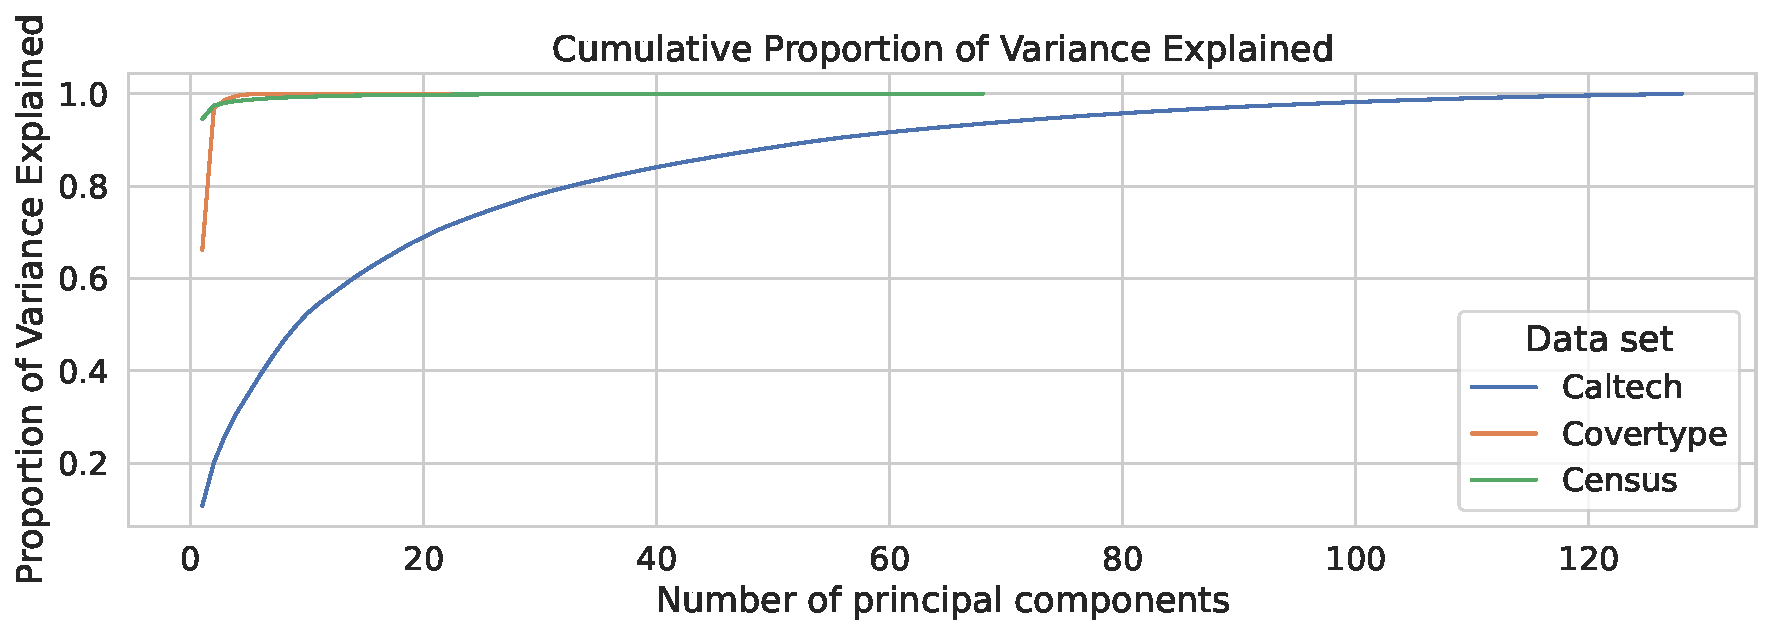
\includegraphics[width=0.9\linewidth]{figures/explained-variance-plot.pdf}
  \caption{The cumulative proportion of explained variance by principal components on \textit{Caltech}, \textit{Covertype}, and \textit{Census}.}
  \label{fig:explained-variance-pca}
\end{figure}

\begin{figure}[!ht]
  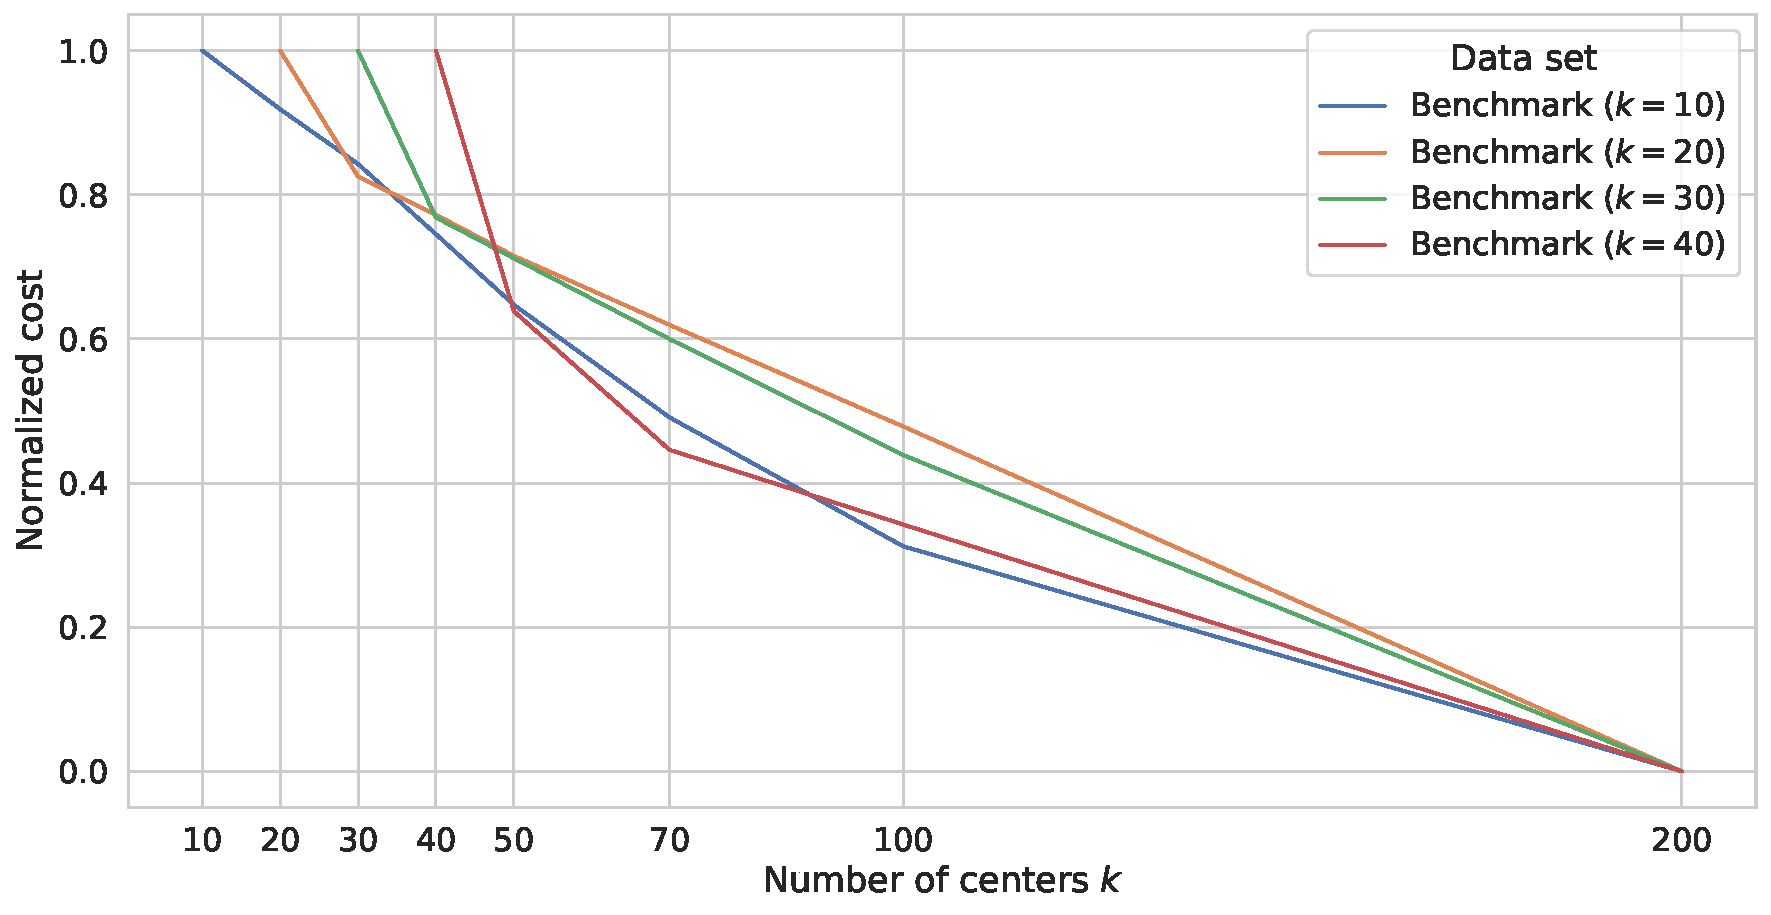
\includegraphics[width=0.9\linewidth]{figures/cost-curves-benchmark.pdf}
  \caption{Shows the clustering costs of four instances of the benchmark framework as a function of the number of centers. In contrast to real-world data sets, the costs do not decrease rapidly as more cluster centers are added.
  }
  \label{fig:cost-curves-benchmark}
\end{figure}

% \begin{figure*}
%  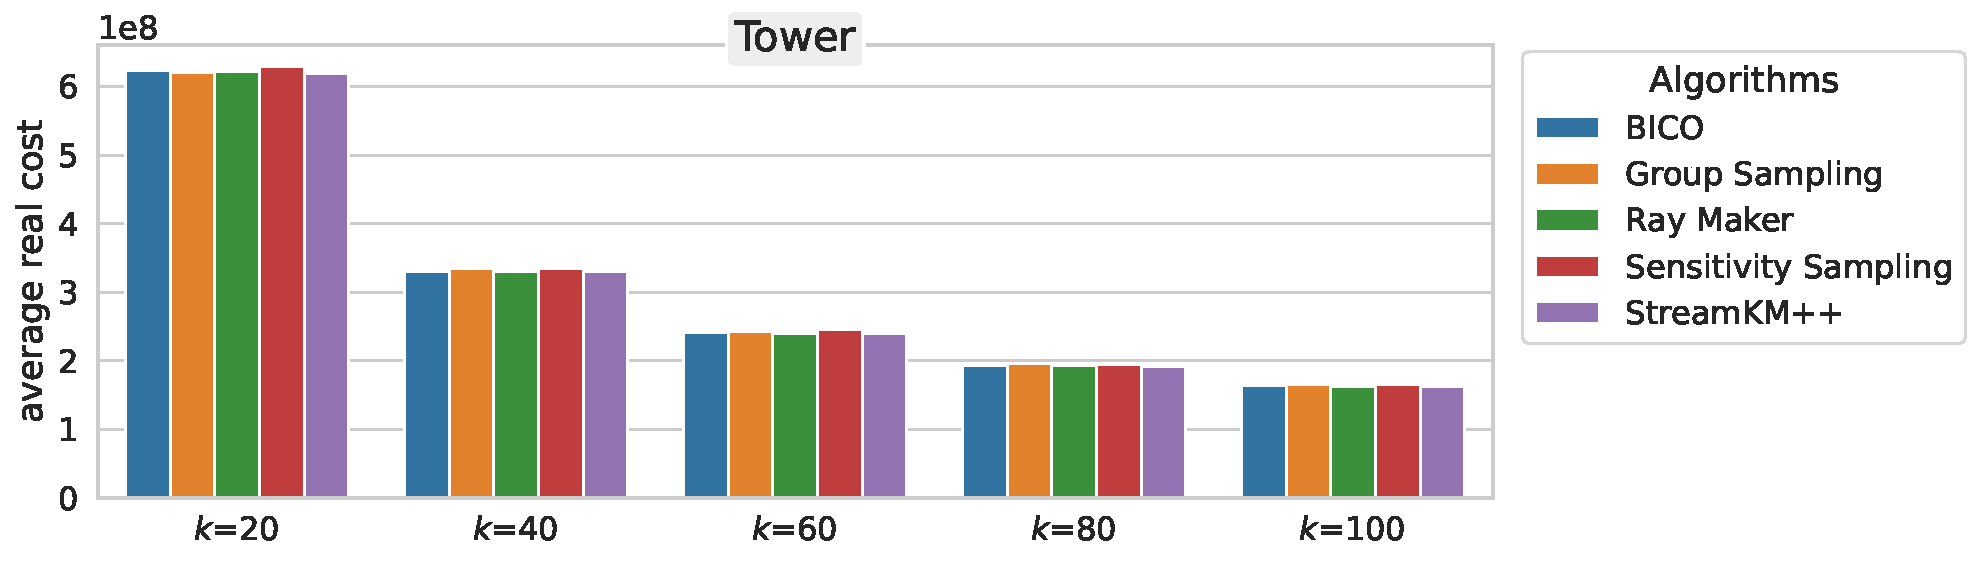
\includegraphics[width=.67\linewidth]{figures/real-costs-Tower.pdf}
%  \newline
%  \subfloat{
%     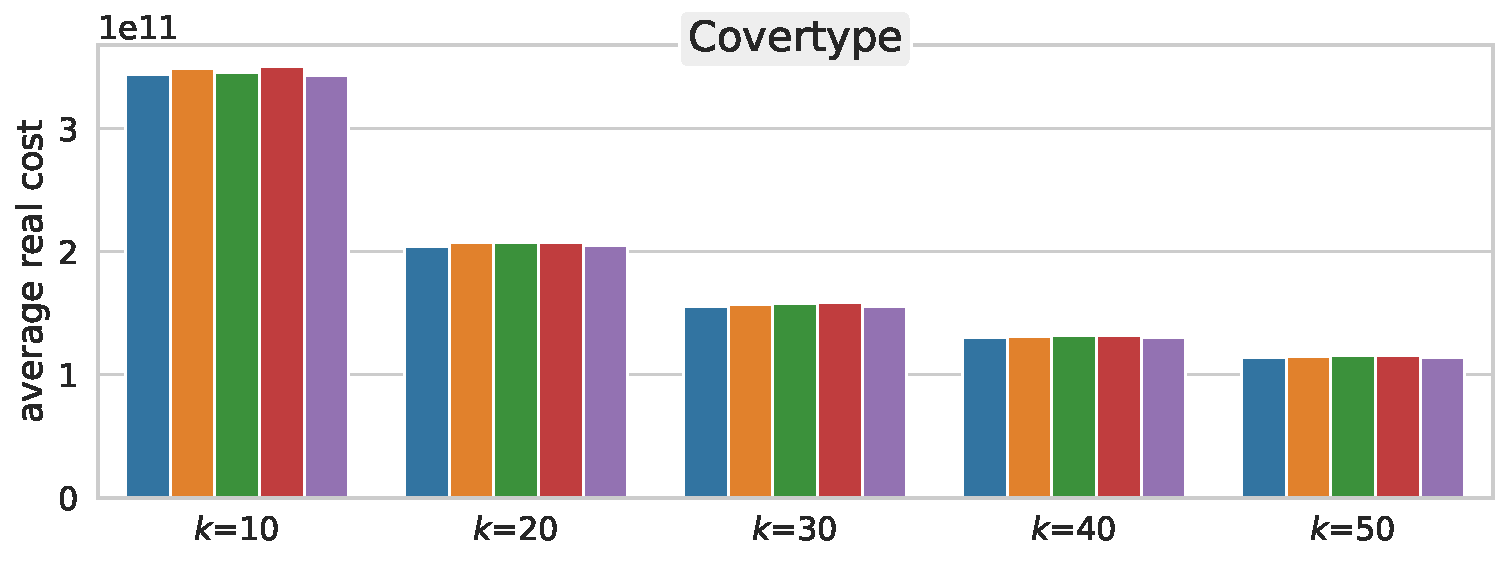
\includegraphics[width=0.5\textwidth]{figures/real-costs-Covertype.pdf}
%  }
%  \subfloat{
%     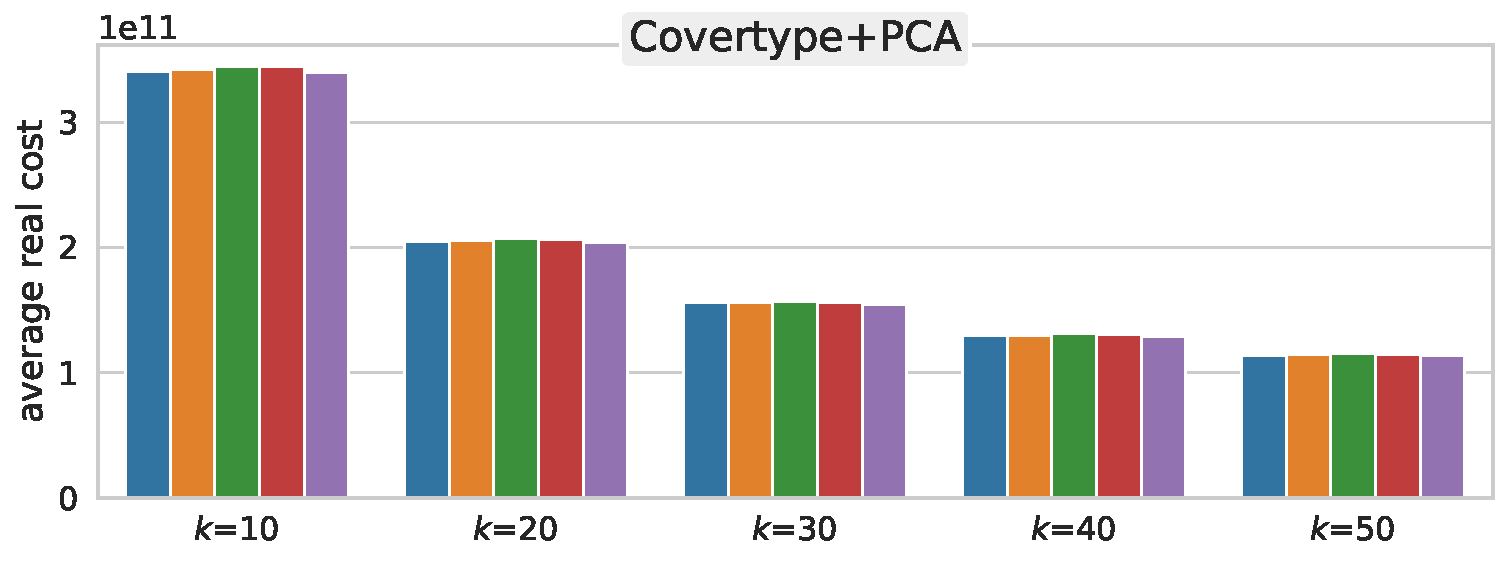
\includegraphics[width=.5\linewidth]{figures/real-costs-Covertype+PCA.pdf}
%  }
%  \newline\newline
%  \subfloat{
%     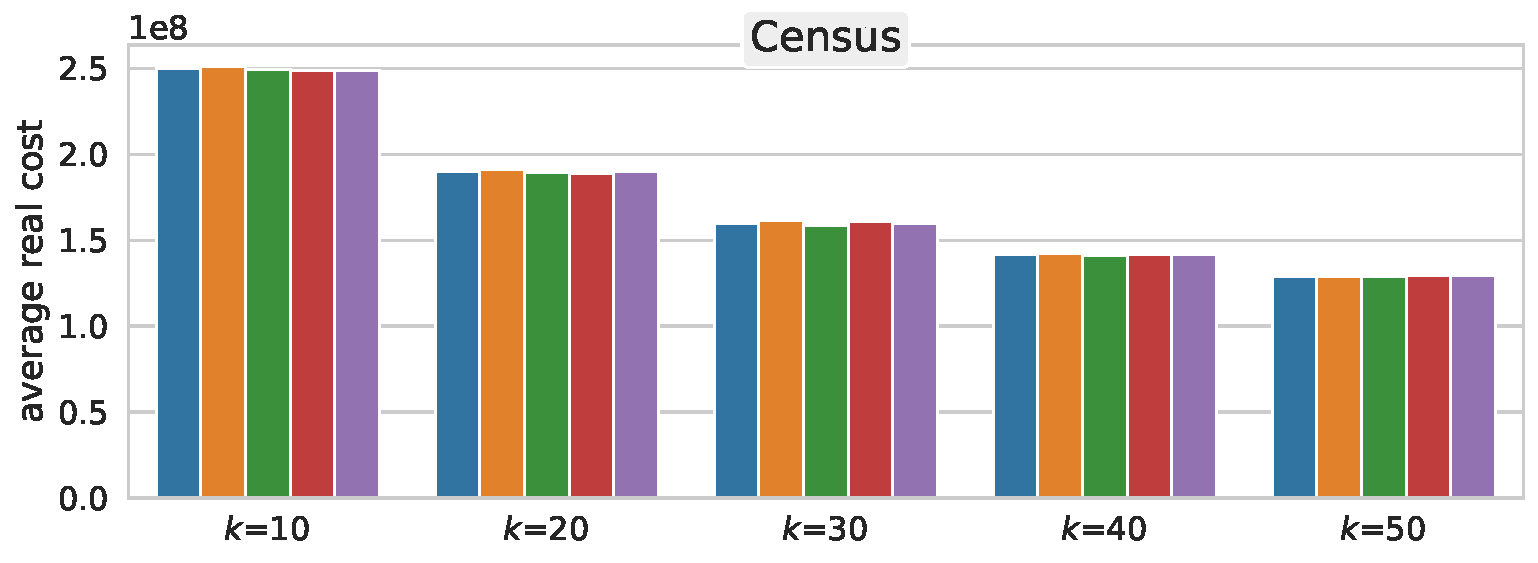
\includegraphics[width=0.5\textwidth]{figures/real-costs-Census.pdf}
%  }
%  \subfloat{
%     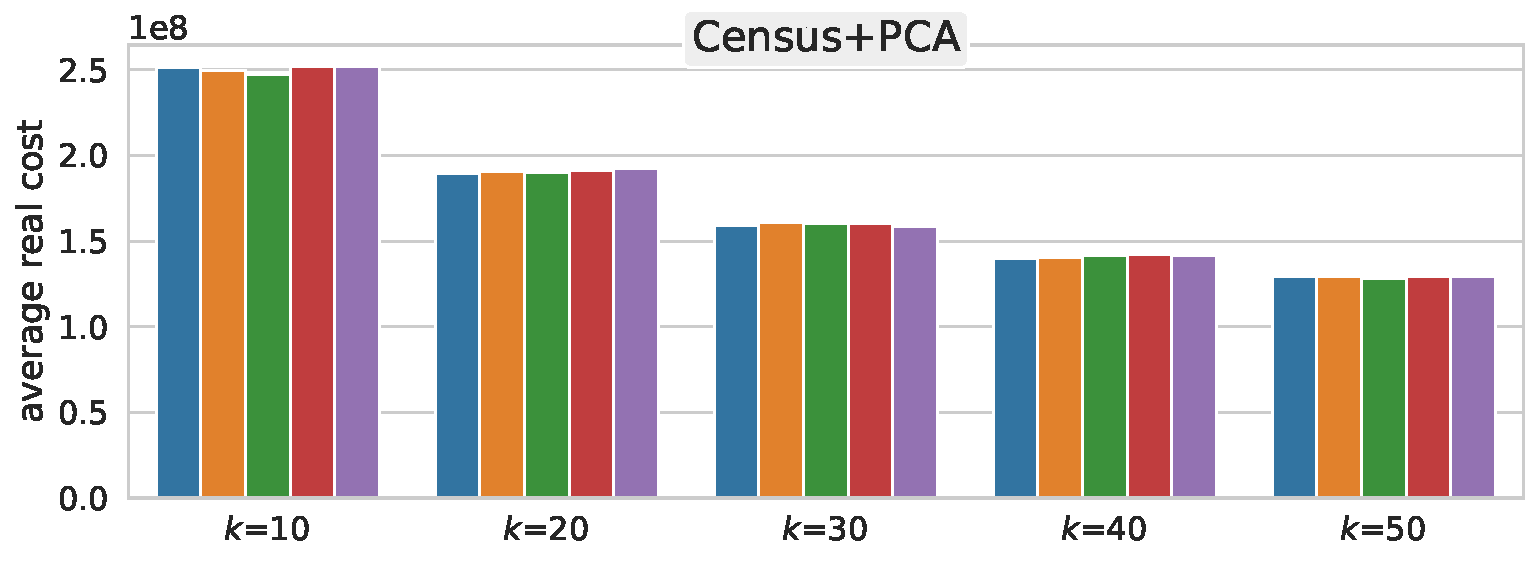
\includegraphics[width=.5\linewidth]{figures/real-costs-Census+PCA.pdf}
%  }
%  \newline\newline
%  \subfloat{
%     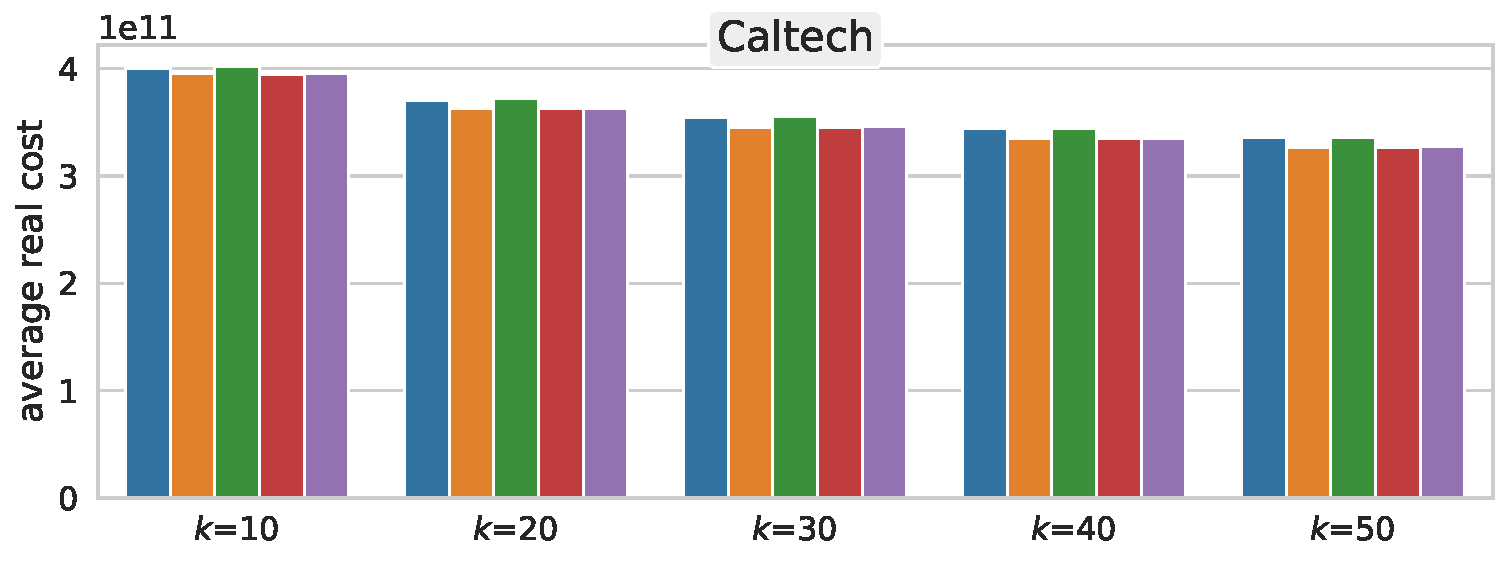
\includegraphics[width=0.5\textwidth]{figures/real-costs-Caltech.pdf}
%  }
%  \subfloat{
%     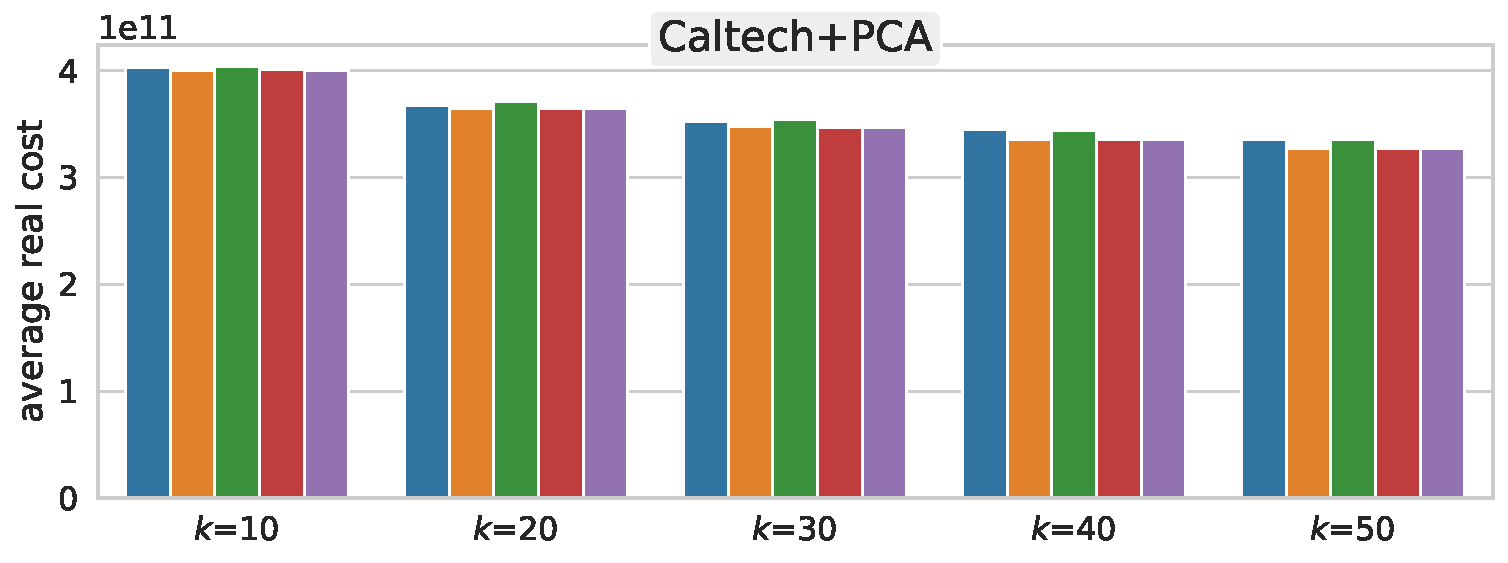
\includegraphics[width=.5\linewidth]{figures/real-costs-Caltech+PCA.pdf}
%  }
%  \newline\newline
%  \subfloat{
%     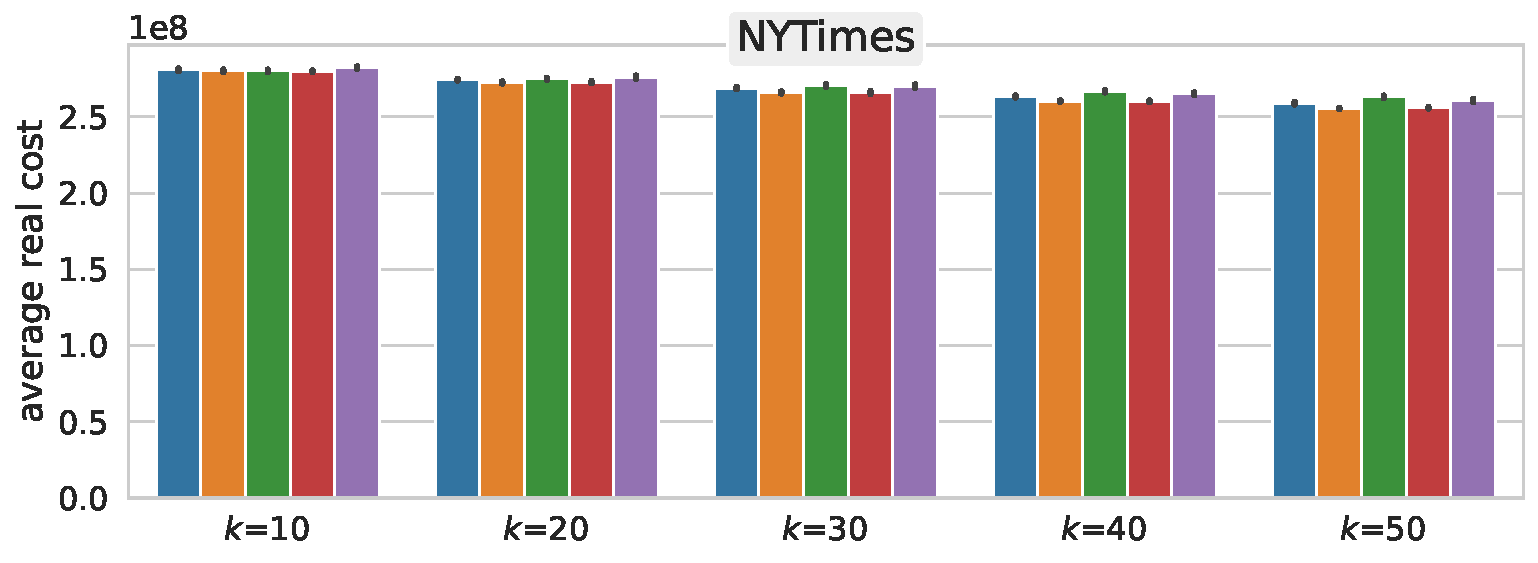
\includegraphics[width=0.5\textwidth]{figures/real-costs-NYTimes.pdf}
%  }
%  \subfloat{
%     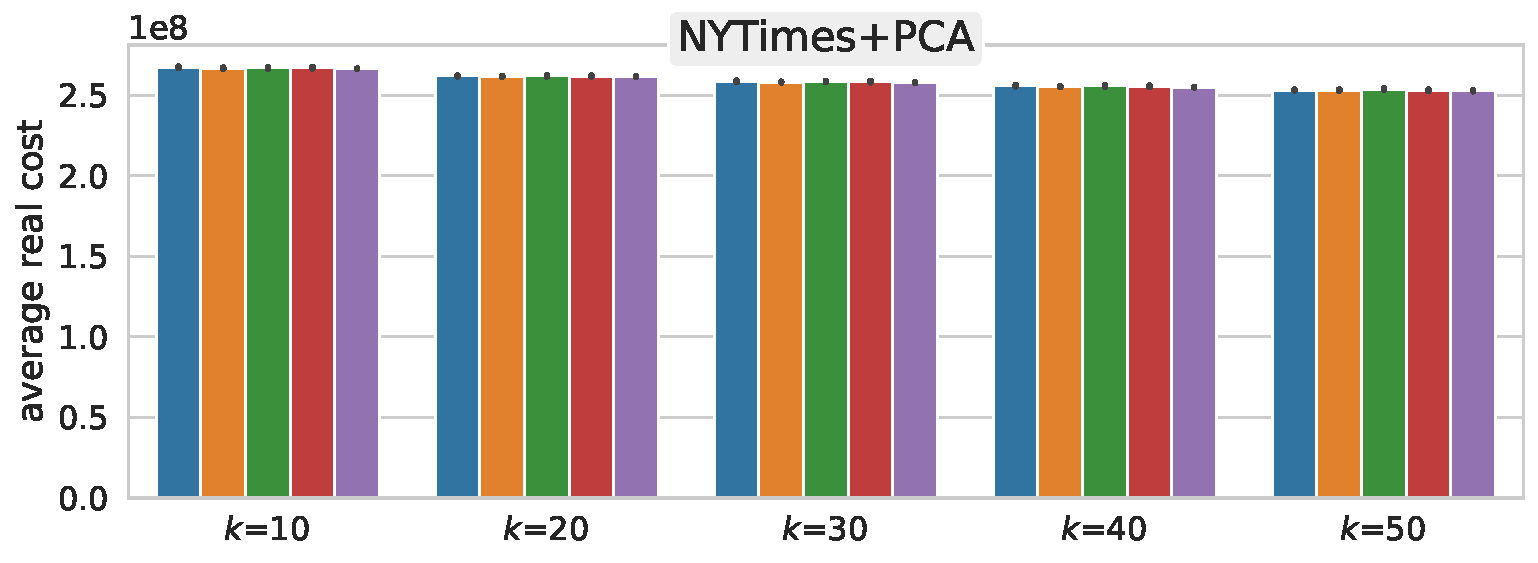
\includegraphics[width=.5\linewidth]{figures/real-costs-NYTimes+PCA.pdf}
%  }
%  \newline\newline
%  \subfloat{
%     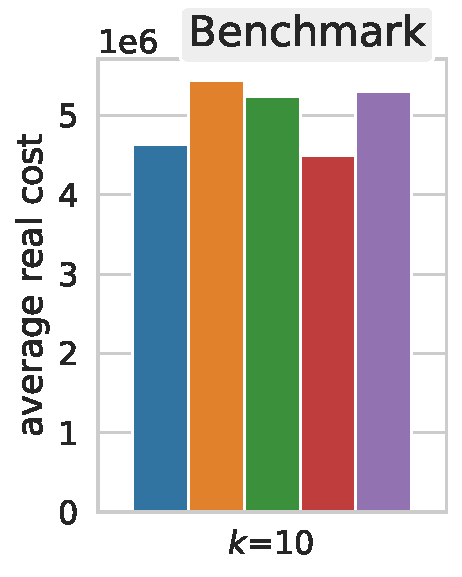
\includegraphics[width=0.15\textwidth]{figures/real-costs-Benchmark-k10.pdf}
%     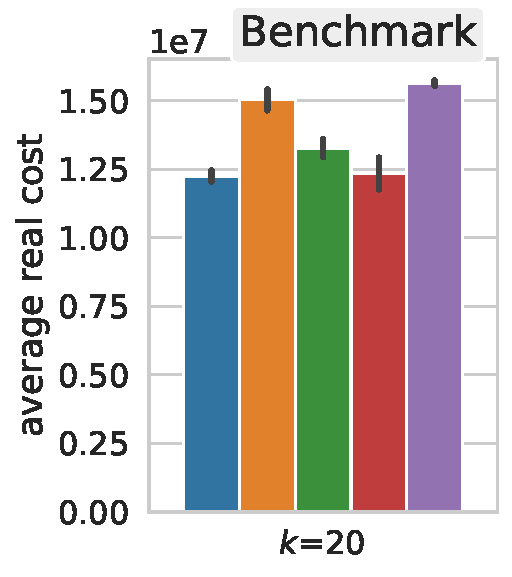
\includegraphics[width=0.165\textwidth]{figures/real-costs-Benchmark-k20.pdf}
%     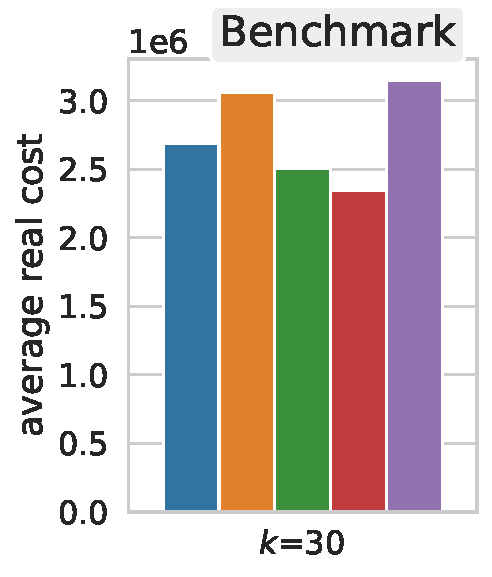
\includegraphics[width=0.16\textwidth]{figures/real-costs-Benchmark-k30.pdf}
%     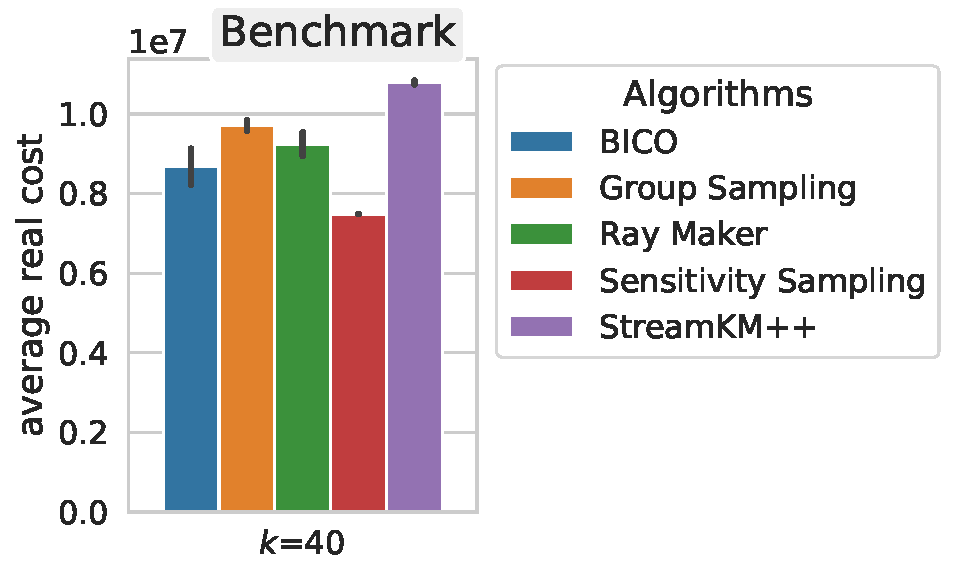
\includegraphics[width=0.31\textwidth]{figures/real-costs-Benchmark-k40.pdf}
%  }
%  \caption{The average costs of running the evaluated coreset algorithms multiple times on different data sets. In general, the five coreset algorithms are able to compute coresets which result in solutions with comparable costs on the different real-world data sets. The differences in cost is more noticeable on the benchmark instances. Here, Senstivity Sampling is the winner because it seems to be better at capturing the correct ``clusters'' inherent in the benchmark instances.}
%  \label{fig:real-costs}
% \end{figure*}





%%
%% Bibliography
%%

%% Please use bibtex, 




\end{document}
